\chapter{Modelling colorectal cancer methylation data with \texttt{methdemon}}
\label{chapter:methylation}
% \large\textbf{OUTLINE}
% \begin{itemize}
%     \item Introduction - methylation modelling literature, data collection
%     \item Results; sections: methdemon recapitulates FMC patterns in crc,
%         evolutionary regimes which explain the data within methdemon,
%         phylogenetic tree analysis
%     \item Discussion
% \end{itemize}

\section{Introduction}
A mathematical model is only as good as its ability to describe its system of
interest. Therefore, in this chapter, I will test how well the
\texttt{methdemon} model describes methylation data sampled from colorectal
cancer (CRC). CRC is the third most common cancer worldwide, with over $40000$
new cases diagnosed in the UK each year on average
\cite{cancer_research_uk_bowel_2021}. The disease is characterised by the
accumulation of genetic and epigenetic mutations in colonic cells
\cite{fleming_colorectal_2012}. The most common type of CRC is adenocarcinoma,
which arises from the epithelial cells lining the colon, covering the majority
of cases. The tumour forms hierarchical cell structures similar to those of
normal tissue, organising into crypt-like glands
\cite{ponz_de_leon_pathology_2001}. The tumour spreads by the process of gland
fission \cite{preston_bottom-up_nodate}, which is similar to the branching
processes seen in normal crypts \cite{almet_multicellular_2018}.

\section{Data collection}
The data used in this study were provided by Dr Darryl Shibata from the Keck
School of Medicine at the University of Southern California. The data consist
of DNA methylation arrays sequenced from multiple glands within colorectal
tumours post-surgery. All samples are anonymised. The arrays were obtained from
bulk samples of tumour glands, which means that the data are nominally not
single-cell resolved. Each tumour sample consists of $8$ glands, with each
gland's array containing some $850000$ CpG sites. The arrays were obtained
using the Illumina Infinium MethylationEPIC BeadChip array. The data were
pre-processed by Dr Shibata to remove low-quality samples and normalise the
arrays. The sample purity was high, with the vast majority of cells in the
samples being tumour cells.

\section{Results}
\subsection{Identification of fCpG loci in colorectal cancer}
The first step in the analysis was to identify the fCpG loci in the data. As
multiple samples come from the same tumour, a larger cohort of samples is
needed to reliably identify fCpG loci using the methods described by
\cite{gabbutt_evolutionary_2023}, i.e. isolating a set of CpG loci which are
the least informative about the methylation state across the cohort. Dr Gabbutt
ran the analysis on colorectal cancer data from the Cancer Genome Atlas (TCGA)
and identified $1258$ fCpG loci. For comparison, I ran a similar analysis only
on the data provided by Dr Shibata and identified a set of some $950$ loci. Of
these, only $120$ were common to both sets. The discrepancy is likely due to
the small sample size of the data provided by Dr Shibata. The fCpG loci
identified in one of the samples are shown in figure \ref{fig:fCpG_loci_M},
with additional figures in appendix \ref{appendix:fCpG_loci}.

\begin{figure}[h]
    \centering
    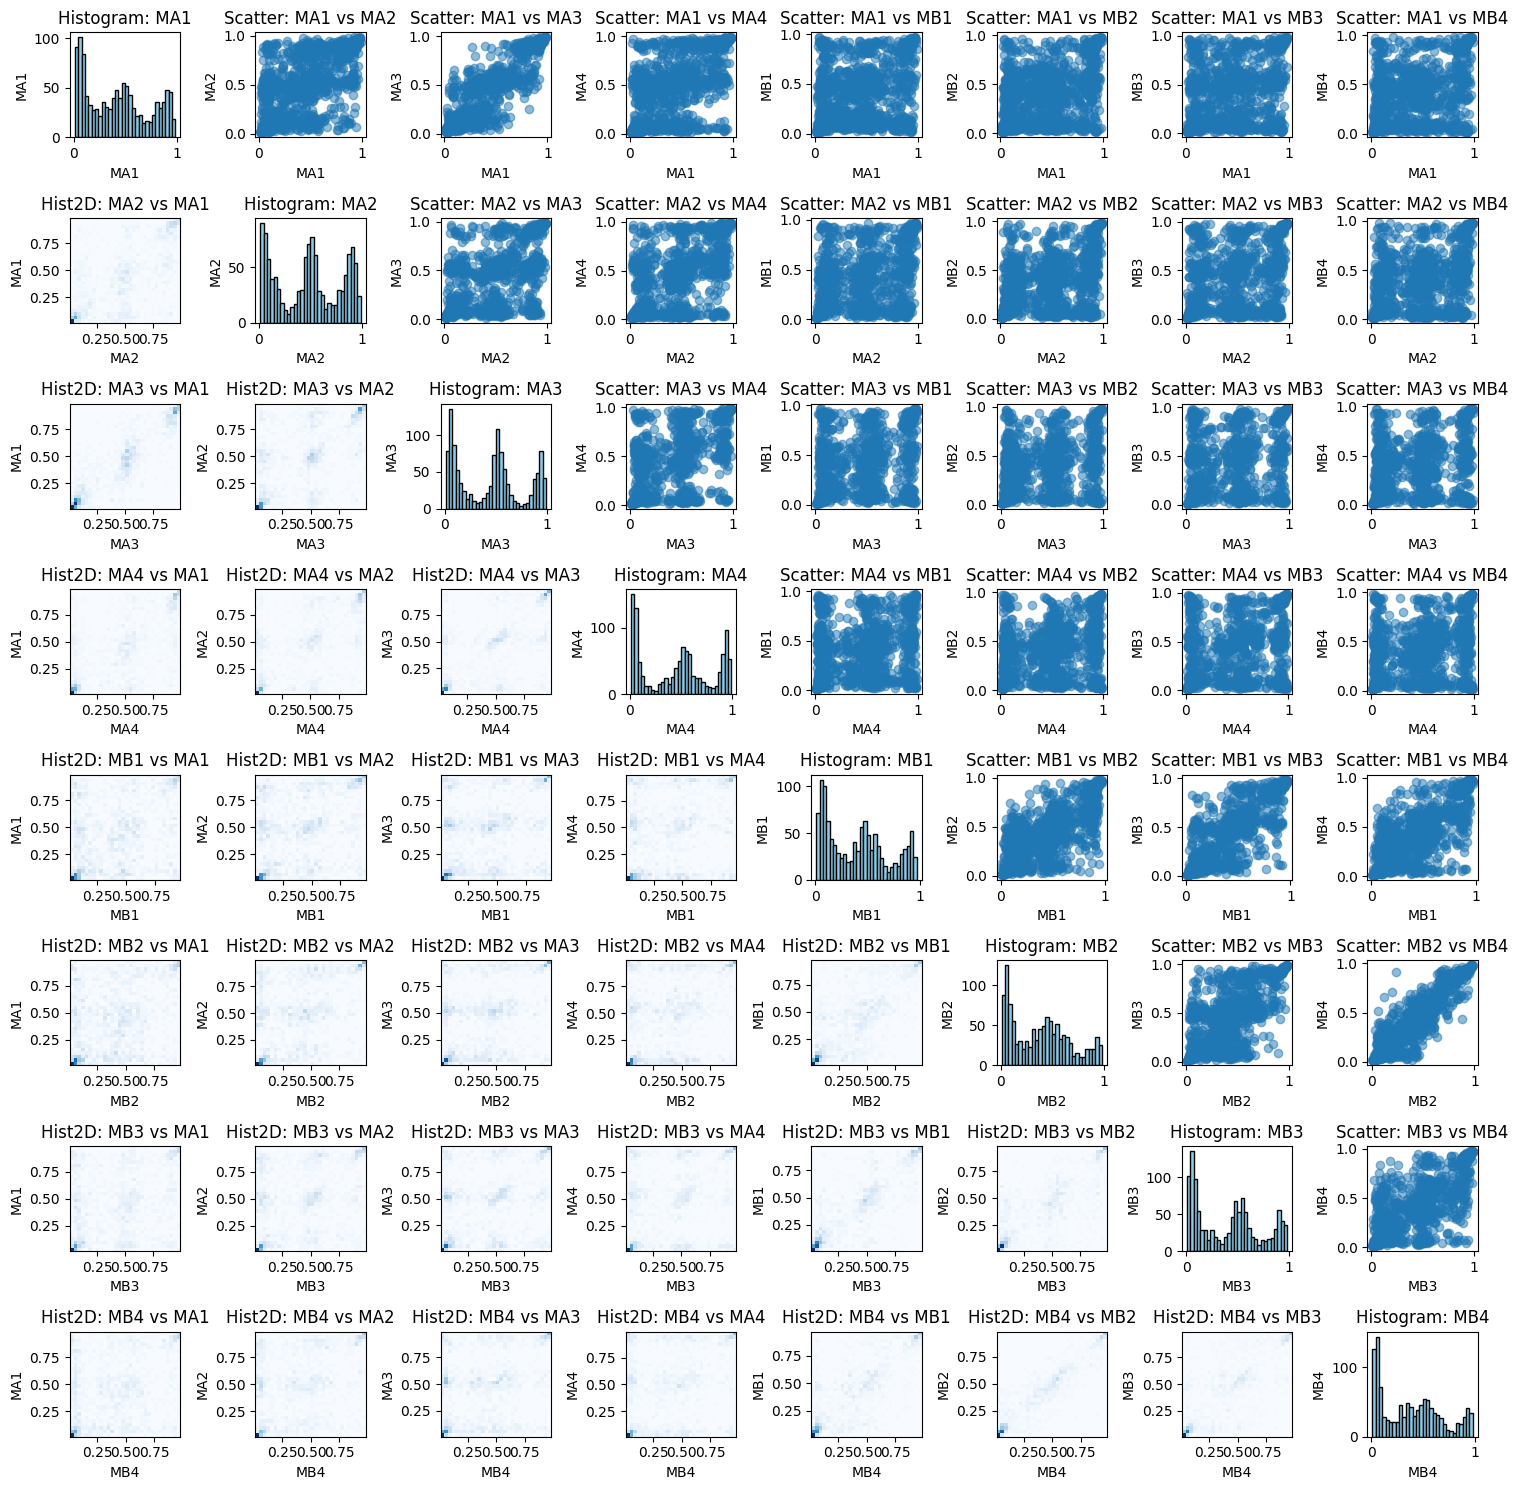
\includegraphics[width=\textwidth]{Chapter_5/figures/fCpG_loci_M.png}
    \caption{Glands from the same side (A, B) of the tumour have more similar
    fCpG arrays than glands from different sides. \textbf{diagonal} ---
    histograms of fCpG arrays for each gland; \textbf{above diagonal} ---
    scatter plots of correlations between glands; \textbf{below diagonal} ---
    $2$D histograms of the above-diagonal plots, showing the density of points.}
    \label{fig:fCpG_loci_M}
\end{figure}

A notable feature of the data is that some samples show a clear bias towards
either hyper- or hypomethylation. This was also the case for fCpG arrays
filtered using only the samples provided by Dr Shibata. This suggests that the
progenitor cell's methylation state is not necessarily random, but could be
affected by internal or external factors. Furthermore, I developed the model
under the assumption that methylation and demethylation rates are constant and
equal across all cells and fCpG loci. While this may be reasonable on average,
there might be mutations which affect these rates, leading to the observed
distributions of fCpG loci states.

\subsection{Spatial proximity predicts similarity between fCpG arrays}
With the assumed hierarchical structure of the tumour in mind, it should make
sense intuitively that glands which are spatially close to each other likely
diverged more recently than glands which are further apart. As a result, they
have spent less time evolving independently and should have more similar fCpG
arrays. To test this hypothesis, I calculated the inter-gland distance matrix
for each tumour sample. The resulting matrices show a clear correlation between
side and distance values. The distance matrix for one of the samples is shown
in figure \ref{fig:gland_dist_M} for tumour M, and in appendix
\ref{appendix:gland_distances} for the other samples.

\begin{figure}[h]
    \centering
    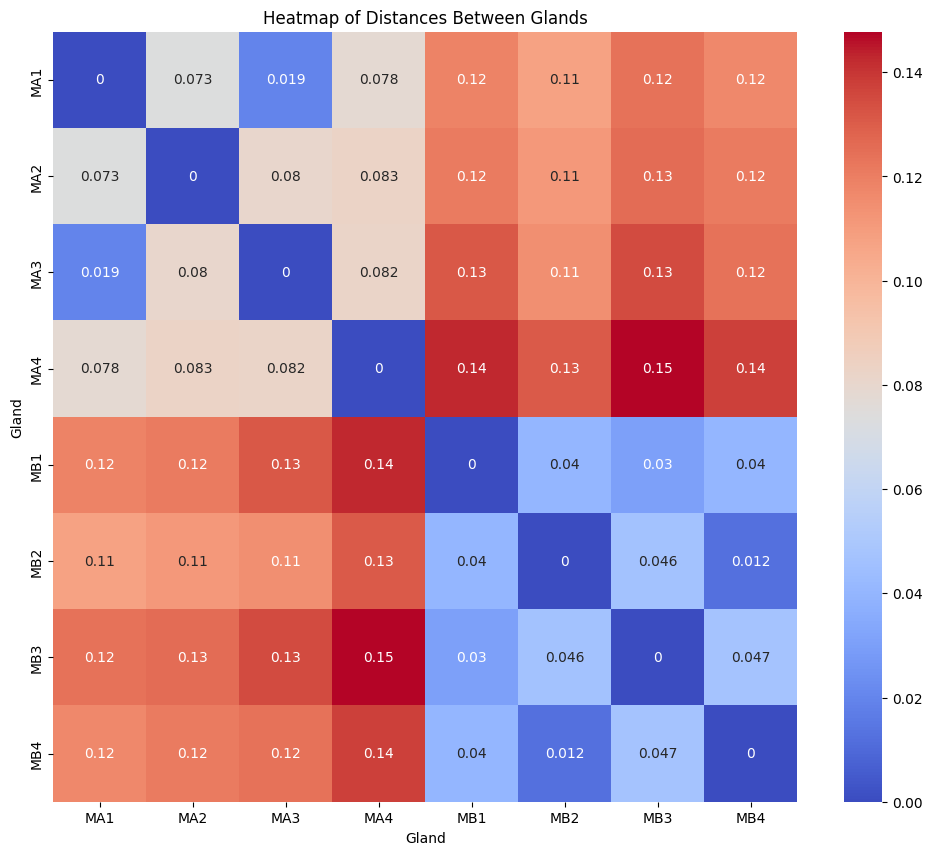
\includegraphics[width=\textwidth]{Chapter_5/figures/gland_dist_M.png}
    \caption{The inter-gland distance matrix for tumour M shows that spatial
    proximity is corelated to similarity between fCpG arrays.}
    \label{fig:gland_dist_M}
\end{figure}

\subsection{Development of the \texttt{methdemon} model}
The \texttt{methdemon} model was developed for the purpose of simulating the
data provided by Dr Shibata. The model's assumptions are based on the general
understanding of colorectal cancer evolution and, translated into the language
of an agent-based model, are as follows:

\begin{enumerate}[(i)]
    \item \textbf{A single cell forms the first gland and initiates tumour
        growth.} This assumption skips over the process of tumorigenesis,
        during which a cell accumulates mutations and becomes malignant
        \cite{tariq_colorectal_2016}. This is a simplification to be sure, but
        a reasonable one, given that the focus of this work is on the
        evolutionary dynamics of the tumour rather than its initiation.
    \item \textbf{The rate of driver mutations is Poisson distributed and
        identical for all cells.} This assumption is consistent with most
        models of tumour evolution \cite{metzcar_review_2019,
        niida_modeling_2021}.
    \item \textbf{The cell population within a gland grows exponentially and is
        well-mixed.} While not necessarily consistent with the biology of a
        solid tumour, this assumption allows for more efficiency in the
        simulation as opposed to a multi-level spatial model. Further, as the
        data discussed in chapter \ref{chapter:methylation} is obtained from
        bulk samples of tumour glands, this assumption is not unreasonable.
        \label{item:well_mixed}
    \item \textbf{Once a gland reaches a certain size, which we call the
        carrying capacity, the population undergoes steady-state turnover
        according to the Moran process.}
    \item \textbf{At carrying capacity, a gland has a certain probability of
        undergoing fission, which splits the gland's population randomly into
        two.} As a consequence of assumption (\ref{item:well_mixed}), fissions
        do not take into account a gland's spatial organisation.
    \item \textbf{Gland fission occurs as a neutral spatial branching process.}
        The previous two assumptions and this one together form the basis of
        the model's spatial dynamics. While there are other mechanisms of
        colorectal adenocarcinoma progression, gland fission is the principal
        way in which the tumour grows \cite{preston_bottom-up_nodate}. The
        assumption of neutrality in the spatial branching process is consistent
        with the findings of \cite{sottoriva_big_2015}. Additionally, this
        assumption is based on the fact that the data used in this study only
        contains information about whether a gland was sample from side A or B,
        without any further spatial information other than the approximate size
        of the full tumour.
\end{enumerate}

\subsection{Higher deme carrying capacity requires stronger selection to
recapitulate the data}
To begin the analysis of cancer data using the \texttt{methdemon} model, I tested the
ranges of parameters based on the assumption that each cancer cell has infinite
proliferative potential. This would mean setting the carrying capacity of a gland
to about $10000$ cells, which is consistent with the size of the glands in the
literature \cite{sottoriva_big_2015} and our data. Due to the glandular
structure of the tumour, this is an effectively neutral model, as selection
acts within glands but not between them, leading to progressive diversification
of the population, as discussed in chapter \ref{chapter:trajectories} and
\cite{noble_spatial_2022}.\par

\begin{figure}[h]
    \centering
    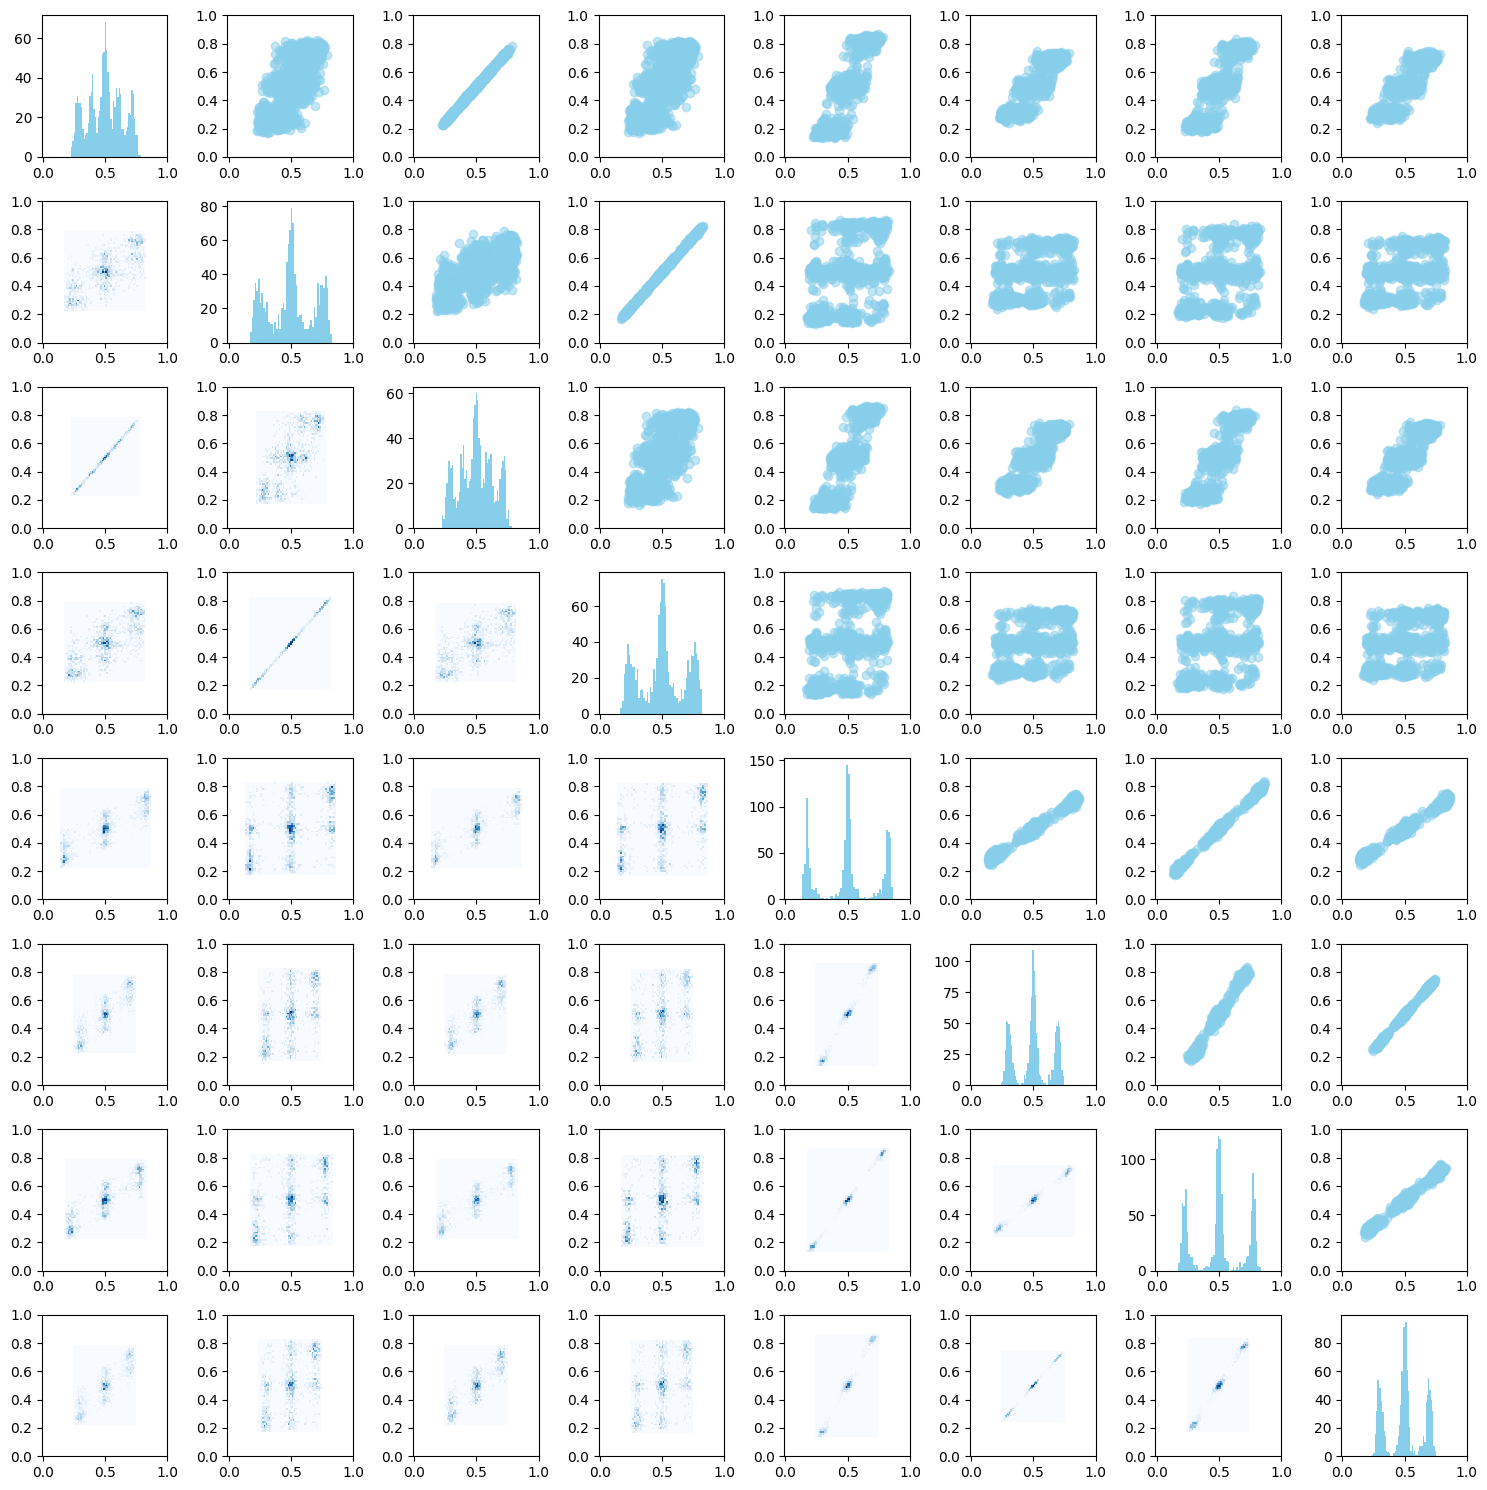
\includegraphics[width=\textwidth]{Chapter_5/figures/10000plot.png}
    \caption{}
    \label{fig:methdemon_weak_selection}
\end{figure}

\begin{figure}[h]
    \centering
    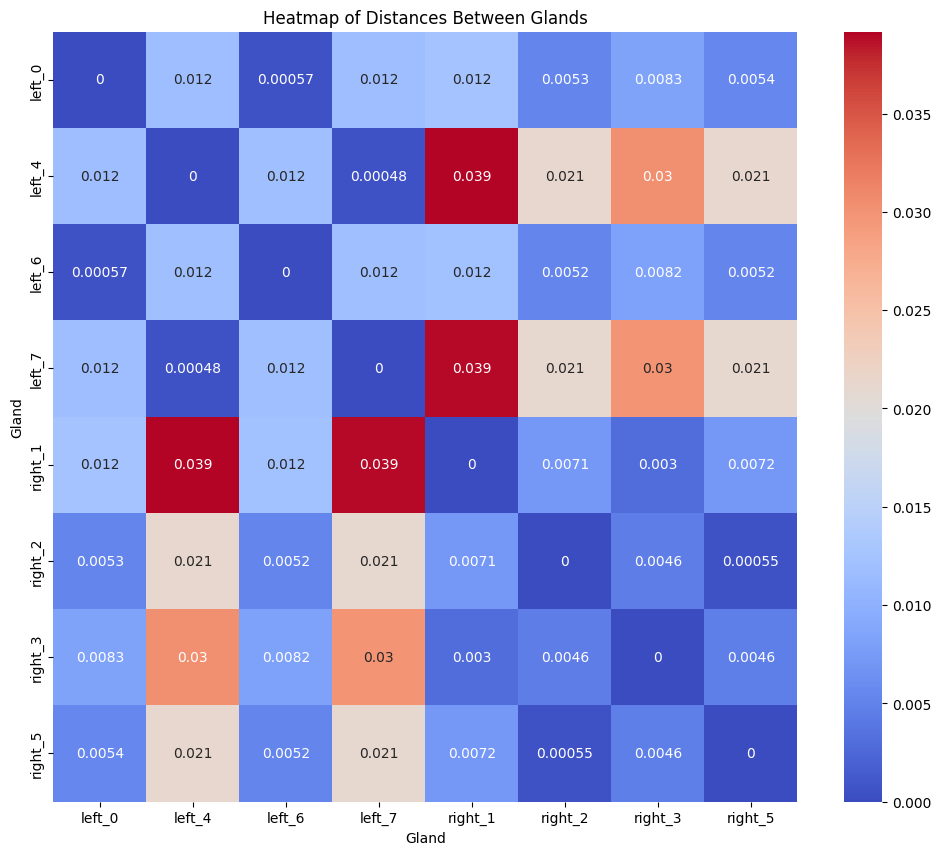
\includegraphics[width=\textwidth]{Chapter_5/figures/10000dist.png}
    \caption{Inter-gland distances for the output fCpG arrays from the
    \texttt{methdemon} model with weak selection.}
    \label{fig:methdemon_weak_dist}
\end{figure}

As a first test, I ran the model with weak selection, $s=0.1$. The resulting
outputs are shown in figures \ref{fig:methdemon_weak_selection} and
\ref{fig:methdemon_weak_dist}. There are a few notable features about the
output fCpG arrays and the distance matrix. The most obvious is that the peaks
associated with homozygous methylation and demethylation states have moved
towards the middle. This is to be expected, as we are treating all $10000$ cells
in a deme as being able to divide ad infinitum, leading to a lot of stochastic
noise. This is a consequence of the time spent in turnover, and is adjusted by
increasing the fission rate. However, the distance matrix shows that the glands
are still very similar to each other, especially when compared to the data. This
is likely due to the fact that there is only a small probability of a partial or
full sweep of a lineage within a gland. The similarity is a consequence of the
large deme carrying capacity, which allows for a lot of stochastic noise to
accumulate over time but lowers the probability of fixation in the weak
selection regime. Increasing the selection coefficient to $s=0.3$ leads to more
divergence between the glands, since emerging lineages are more likely to fully
or partially sweep the gland's population and establish more distinct fCpG
arrays between glands. However, as discussed in chapter \ref{chapter:methdemon},
strong selection can quickly become problematic in an ABM like this due to the
accumulation of advantageous drivers. An example of strong selection at deme
size $10000$ is in appendix \ref{appendix:inference}. \par
Considering that the number of stem cells in a normal crypt is on the order of
$10$ \cite{gehart_tales_2019, gabbutt_fluctuating_2022}, with the total number
of cells in a crypt being on the order of $1000$, I next tested the model with
a deme carrying capacity of $100$ i.e. about $1\%$ of the total cell population
in the gland. The currently available data supports this percentage as a
reasonable estimate of the proportion of cancer stem cells (CSCs) in colorectal
cancer \cite{obrien_human_2007, munro_cancer_2018}. In this case, the model's
outputs are as expected, with the fCpG arrays diverging over time even with no
or weak selection. Examples are shown in figures
\ref{fig:methdemon_weak_selection_small} and
\ref{fig:methdemon_weak_dist_small}.

\begin{figure}[h]
    \centering
    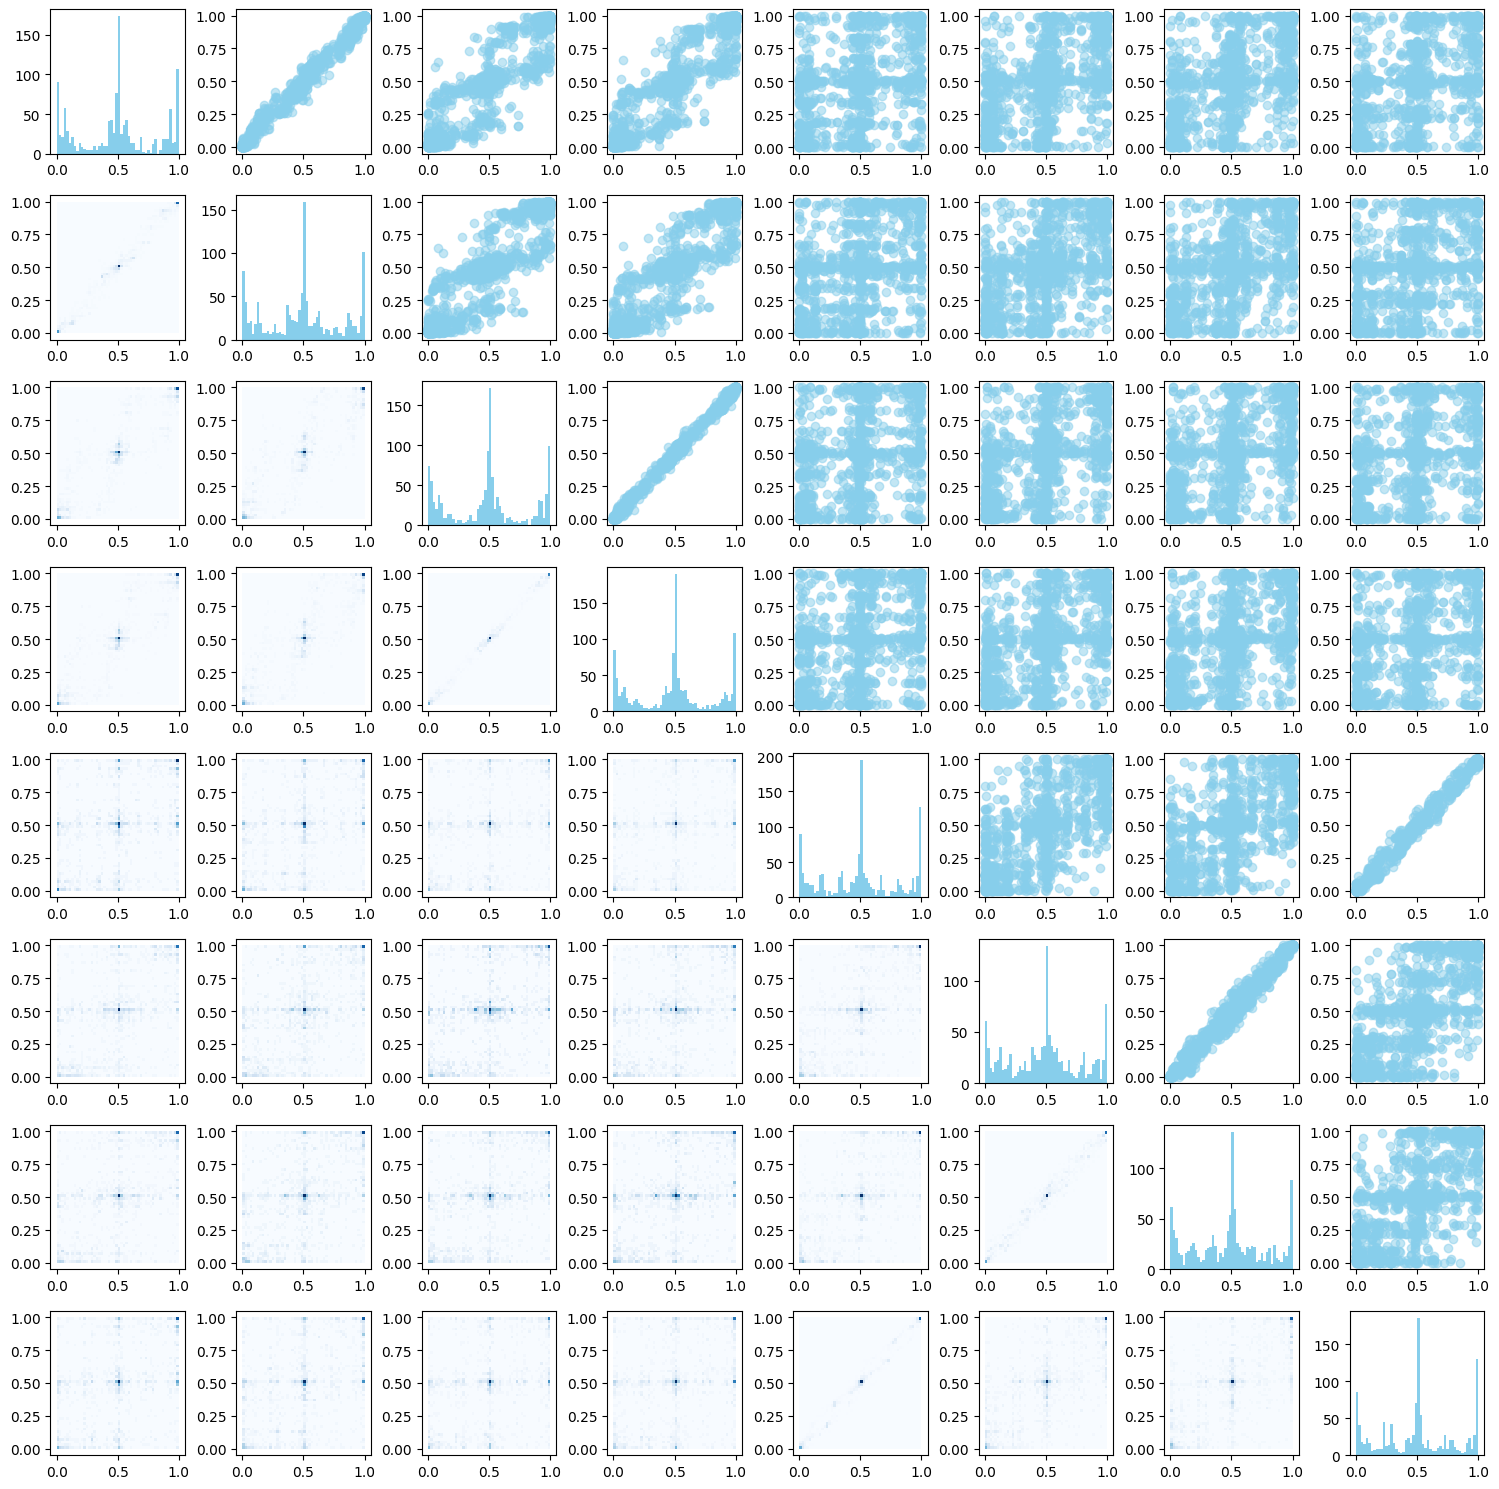
\includegraphics[width=\textwidth]{Chapter_5/figures/100plot.png}
    \caption{Output fCpG arrays from the \texttt{methdemon} model with weak
    selection and deme carrying capacity $100$ reflect the data better than
    larger deme carrying capacity.}
    \label{fig:methdemon_weak_selection_small}
\end{figure}

\begin{figure}[h]
    \centering
    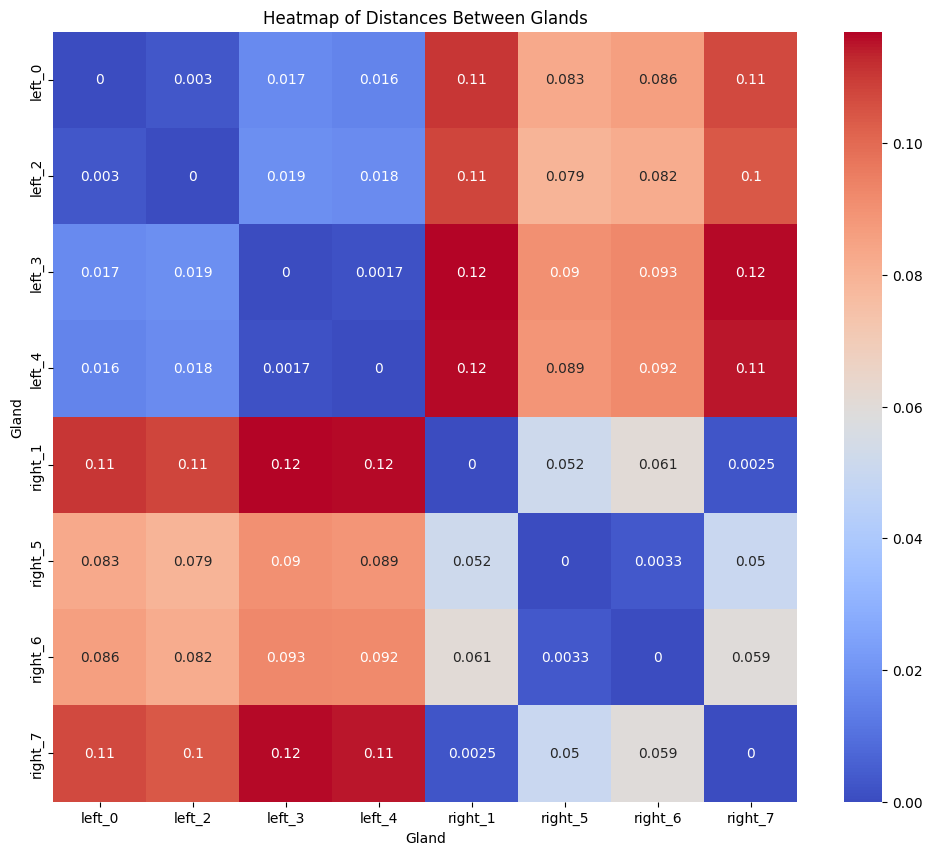
\includegraphics[width=\textwidth]{Chapter_5/figures/100dist.png}
    \caption{Inter-gland distance matrix corresponding to the run from figure
    \ref{fig:methdemon_weak_selection_small}.}
    \label{fig:methdemon_weak_dist_small}
\end{figure}
\clearpage

\subsection{Parameter inference from colorectal cancer data}
\subsubsection{Regular model}
Having established \texttt{methdemon}'s ability to output data which resembles
observations, I next attempted to fit the model to the colorectal cancer data.
For this, I used the ABC workflow described in chapter \ref{chapter:methdemon}.
Considering the results of the previous section, I set the deme carrying
capacity to $100$ for all inference runs. I made this choice as there is no
evidence to suggest different numbers of stem cells across tumours or even
glands within a tumour. Furthermore, having the deme carrying capacity as a free
parameter would slow down the inference process significantly.
In the first instance, I ran the inference with parameter ranges given in table
\ref{tab:inf_ranges}. The results of the inference are shown in figure
\ref{fig:inference_1}, with more details in appendix \ref{appendix:inference}.

\begin{table}[ht]
\centering
\begin{tabular}{|l|l|l|}
\hline
Parameter & Prior \\
\hline
methylation rate & $U(0, 0.1)$ \\
demethylation rate & $U(0, 0.1)$ \\
fission rate & $U(10^{-4}, 10^{-2})$ \\
driver mutation rate & $U(0, 10^{-2})$ \\
selective advantage & $U(0, 0.2)$ \\
\hline
\end{tabular}
\caption{Parameter priors for the first inference run.}
\label{tab:inf_ranges}
\end{table}

The first inference run did produce some results, but the posterior
distributions of some parameters remained broad. There are a few possible
reasons for this. Firstly, I intentianally used overly broad priors to see how
well the ABC workflow would delineate the parameter space. This choice makes the
inference process more dificult, as the prior distributions are not informative
and the parameter space is large. However, it allows for future runs with more
informative priors. The second reason may just be that the model is not able to
recover all of the parameters in its current form. Selective advantage and
driver mutation rate in particular seem to be difficult to infer for the model.
This could be due to the signature of selection being too weak in the model or
data (or both). It could also be down to the distance functions in the ABC
rejection step not being able to capture the differences between the arrays
well enough. Either way, the results prompted further testing with the important
change of log-transforming the parameters. This change allows for more efficient
exploration of the parameter space, as parameters are sampled on the same scale
and steps between generations will cover more of the space.

\begin{figure}[h]
    \centering
    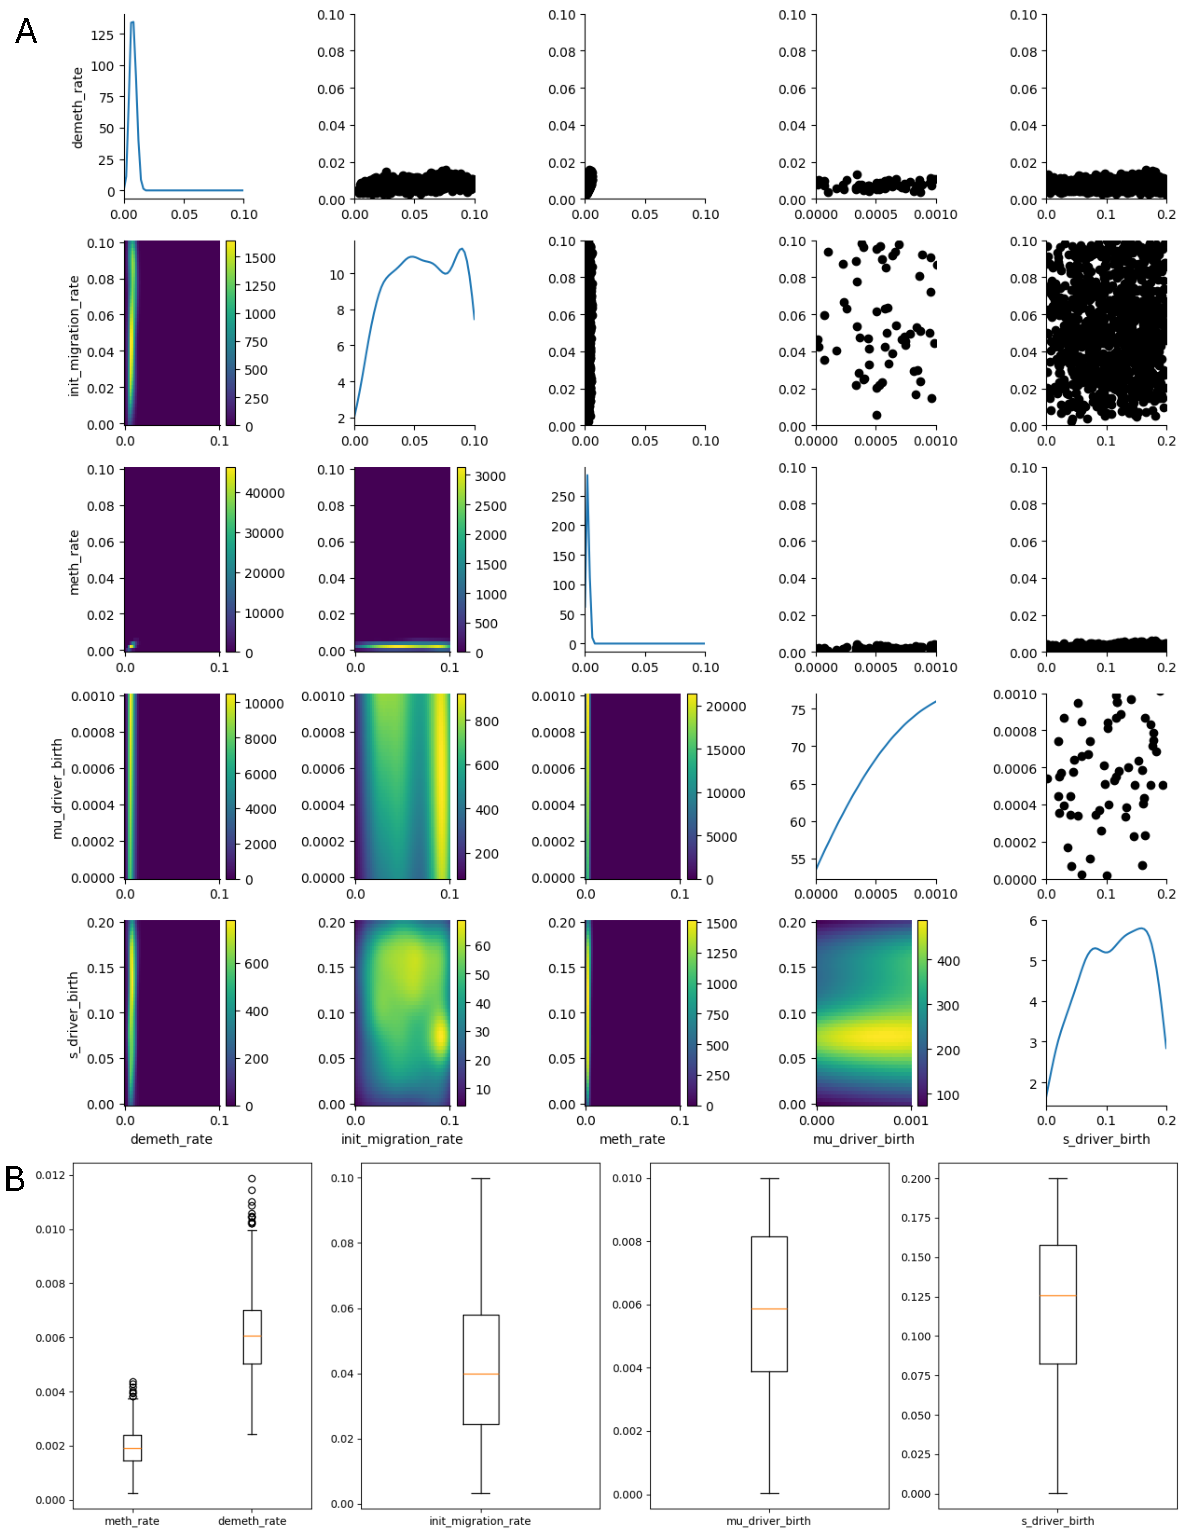
\includegraphics[width=\textwidth]{Chapter_5/figures/inference_raw/inference_1.pdf}
    \caption{Using absolute parameter values in the inference process leads to
    less efficient inference. \textbf{A} --- posterior distributions of fCpG
    fluctuation rates have narrowed down rapidly, but other parameters'
    posteriors remain broad. \textbf{B} --- box plots of the posteriors show
    that the model is not able to resolve the effects of selection from the
    data, and leaves a lot of uncertainty in the fission rates.}
    \label{fig:inference_1}
\end{figure}
\clearpage

\subsubsection{Log-transformed model}
The second inference run was done with similar parameter ranges as the first.
The log-transformed parameter ranges are give in table \ref{tab:inf_ranges_log}
and the results of the inference are shown in figure \ref{fig:inference_2}, with
more details in appendix \ref{appendix:inference}. All log transformations were
done with base $10$.

\begin{table}[ht]
\centering
\begin{tabular}{|l|l|l|}
\hline
Parameter & Prior \\
\hline
log methylation rate & $U(-4, -2)$ \\
log demethylation rate & $U(-4, -2)$\\
log fission rate & $U(-3.3, -1)$\\
log driver mutation rate & $U(-5, -2)$\\
selective advantage & $U(0, 0.2)$\\
\hline
\end{tabular}
\caption{Log-transformed priors for the second inference run.}
\label{tab:inf_ranges_log}
\end{table}

The results of the second inference run are more promising than the first, with
the fission rate posterior distribution being considerably narrower. However,
selection and driver mutation rate are still difficult to narrow down. This
further supports the idea that the model is not able to detect weak selection
at the gland level.

\begin{figure}[h]
    \centering
    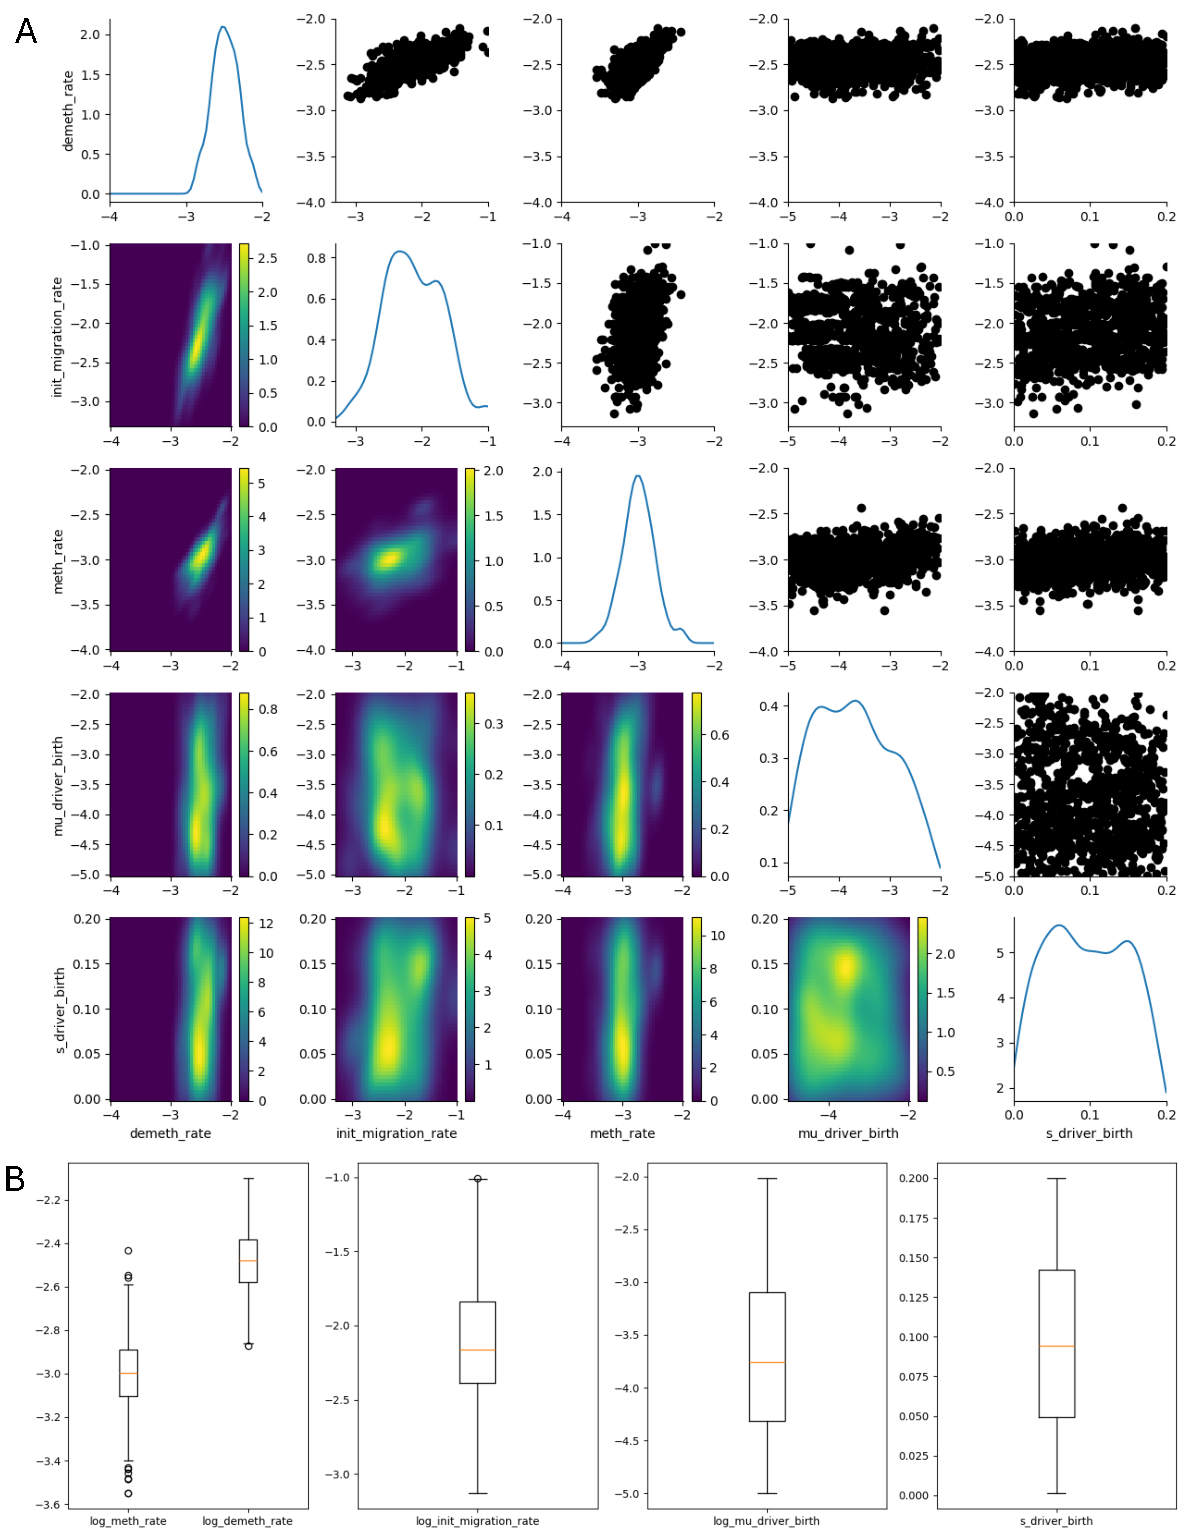
\includegraphics[width=\textwidth]{Chapter_5/figures/inference_2.pdf}
    \caption{STILL RUNNING ON THE CLUSTER.}
    \label{fig:inference_2}
\end{figure}
\clearpage

\subsection{Fast- and slow-growing tumours}
The data provided by Dr Shibata contains samples from different patients, with
each tumour being potentially at a different stage of growth. From exploratory
analysis, it seems that some tumours are growing faster than others, if we work
under the assumption that gland fission is the only mechanism of growth. This
hypothesis is supported by the inference results, as samples with higher values
in the inter-gland distance matrix tend to grow slower, and ones where gland
fCpG arrays are more similar have grown faster. The inferred median fission
rates are shown in table \ref{tab:fission_rates}.
\begin{table}[ht]
\centering
\begin{tabular}{|l|l|}
\hline
Tumour & Median fission rate \\
\hline
\end{tabular}
\caption{Median fission rates for each tumour.}
\label{tab:fission_rates}
\end{table}

\section{Discussion}
% \begin{itemize}
%     \item $1$D model recaps FMC patterns in CRC
%     \item colorectal cancer fcpg data can be explained by effectively neutral
%         evolutionary regimes
%     \item further work - likelihood-based inference, large scale modelling of
%         colorectal cancer
%     \item initial conditions - does a fully random initial array make sense in
%         the context of patterns in data? some tumours do indeed look like they
%         simply have unequal meth and demeth rates, but others look like they
%         started hypo- or hypermethylated.
% \end{itemize}

In this chapter, I tested the \texttt{methdemon} model on colorectal cancer
methylation data using approximate Bayesian computation. The model was able to
recapitulate the patterns observed in the data, and the inferred parameters lay
within reasonable ranges. However, the model struggled to infer the selection
coefficient and the driver mutation rate. This could be due to the signature of
selection being too weak in the model or data, or the distance functions in the
ABC rejection step not being fine-grained enough to detect the differences
between evolutionary modes. Having said that, the results do support an
effectively neutral evolutionary mode of colorectal cancer growth, with the
effects of selection constrained to within glands. Furthermore, it seems clear
that multi-site sequencing of methylation arrays from solid tumours can be used
to draw inferences about the evolutionary dynamics of the tumour, and warrants
further investigation with a more sophisticated model.


% \section{Background on colorectal cancer --- model assumptions}

% \subsection{Colorectal cancer evolution}\label{section:assumptions:general}

% The most common type of colorectal cancer is adenocarcinoma, which arises from
% the epithelial cells lining the colon, covering more than $90\%$ of cases. Most
% diagnosed colorectal cancers are moderately to well differentiated, meaning
% that at least $50\%$ of the tumour's cells form glands
% \cite{fleming_colorectal_2012}. As it is a solid tumour, one cannot ignore the
% spatial organisation of the cells. Its origin, tumorigenesis, follows an
% accumulation of mutations in a cell's DNA, which leads to the cell's
% transformation from a healthy to malignant cell \cite{fearon_genetic_1990}.
% Once the malignancy is established, the tumour forms hierarchical cell
% structures similar to those of normal tissue \cite{cernat_colorectal_2014},
% organising into crypt-like glands. The tumour spreads by the process of gland
% fission, which happens when a gland's population grows large enough to split
% into two glands \cite{preston_bottom-up_2003}. \par Translated into the
% language of an agent-based model, I can write down the initial assumptions as
% follows:

% \section{Introduction}
% \begin{itemize}
%     \item go over literature regarding colorectal adenocarcinoma evolution (pathology, big bang, etc.)
%     \item discuss the relevant parts of the literature in the context of modelling
%     \item explain how the data were collected (ask Darryl)
% \end{itemize}
% The model discussed in this report is the $1$D version of the agent-based model \texttt{demon} developed by Rob. All rates and are given relative to the birth rate which is assumed to be equal to $1$ (as per the Gillespie algorithm).
% \section{Results}
% I performed the preliminary sensitivity analysis on a small set of simulations, more as a sanity check than a robust test. However, the results are interesting as the model is more sensitive to some parameters than expected. The parameters, checked are ones controlling selective advantage, driver mutation rates, fCpG flipping probabilities, and gland fission rates.
% \subsection{A note on the fully neutral model}
% As discussed in previous meetings, the fully neutral model does not behave as expected. Instead, its outputs look like they are just oscillations around the initial fCpG array. This, I think, is due to the lack any preference for one lineage over any other within a gland, leading to a decoherence of the arrays after a long period of turnover, but without any resolution in space/time. However, even with selective advantage for driver mutations within glands, the glands themselves undergo fission in space neutrally as there is no competition for space in the model. The limitations of this assumption need to be discussed, but it seems reasonable for now.

% \subsection{Selective advantage}
% The selective advantage, accounted for in the model as
% \begin{equation}
%     \lambda' = \lambda\left(1 + s\left(\frac{\lambda}{\lambda_{max}}\right)\epsilon\right),
% \end{equation}
% where $\lambda$ is the birth rate before mutation, $\lambda'$ is the birth rate after mutation, $\lambda_{max}$ is the maximal allowed birth rate, and $\epsilon$ is a unit exponentially distributed value. The values of $s$ tested were $0.1$, $0.2$, and $0.3$ with the other parameters kept at values given in table \ref{tab:parameters}.
% \begin{figure}[h]
%     \centering
%     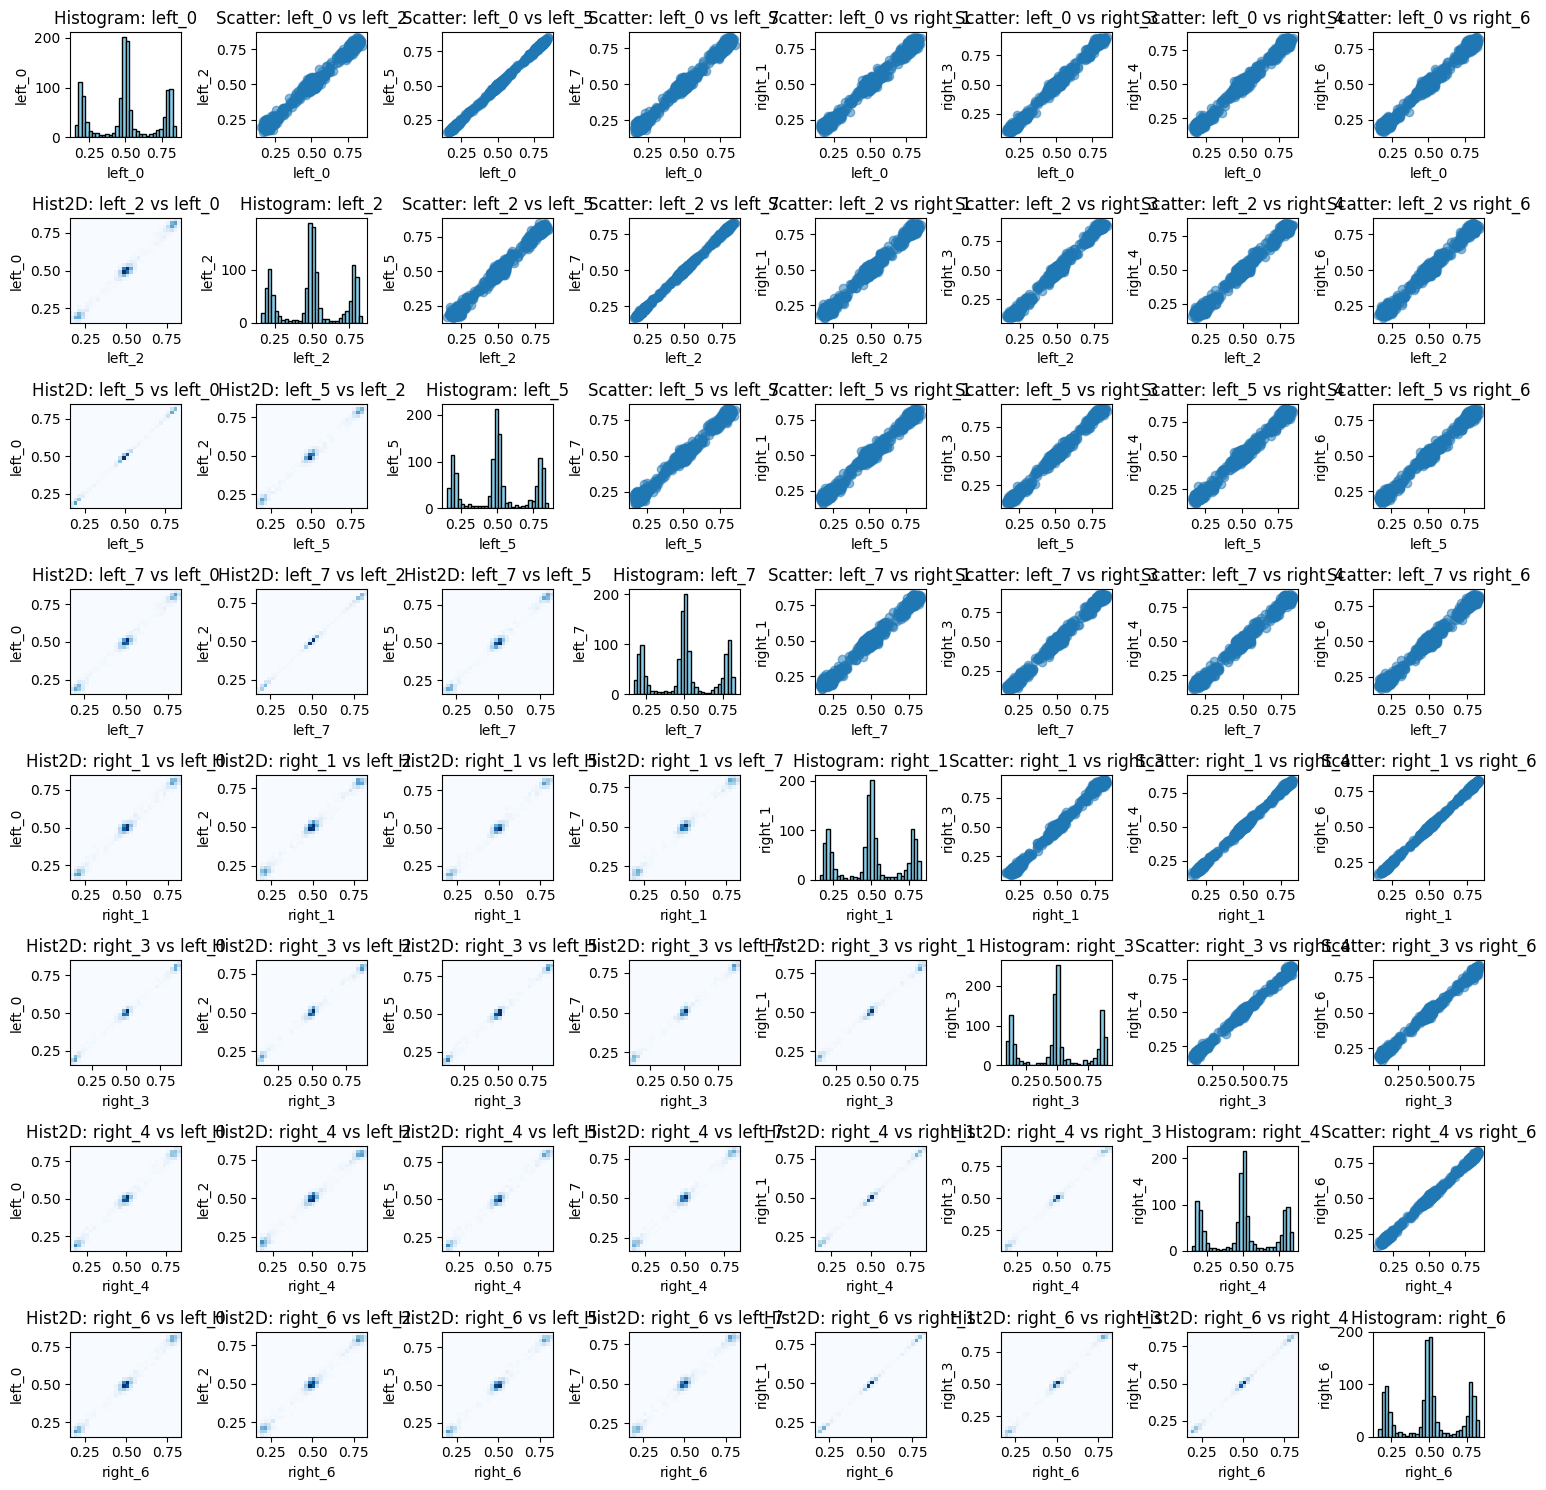
\includegraphics[width=\textwidth]{Chapter_5/figures/sensitivity_selective_advantage1.png}
%     \caption{correlation scatter plots, gland histograms and correlation heatmaps for $s=0.1$.}
%     \label{fig:sensitivity_selective_advantage1}
% \end{figure}
% \begin{figure}[h]
%     \centering
%     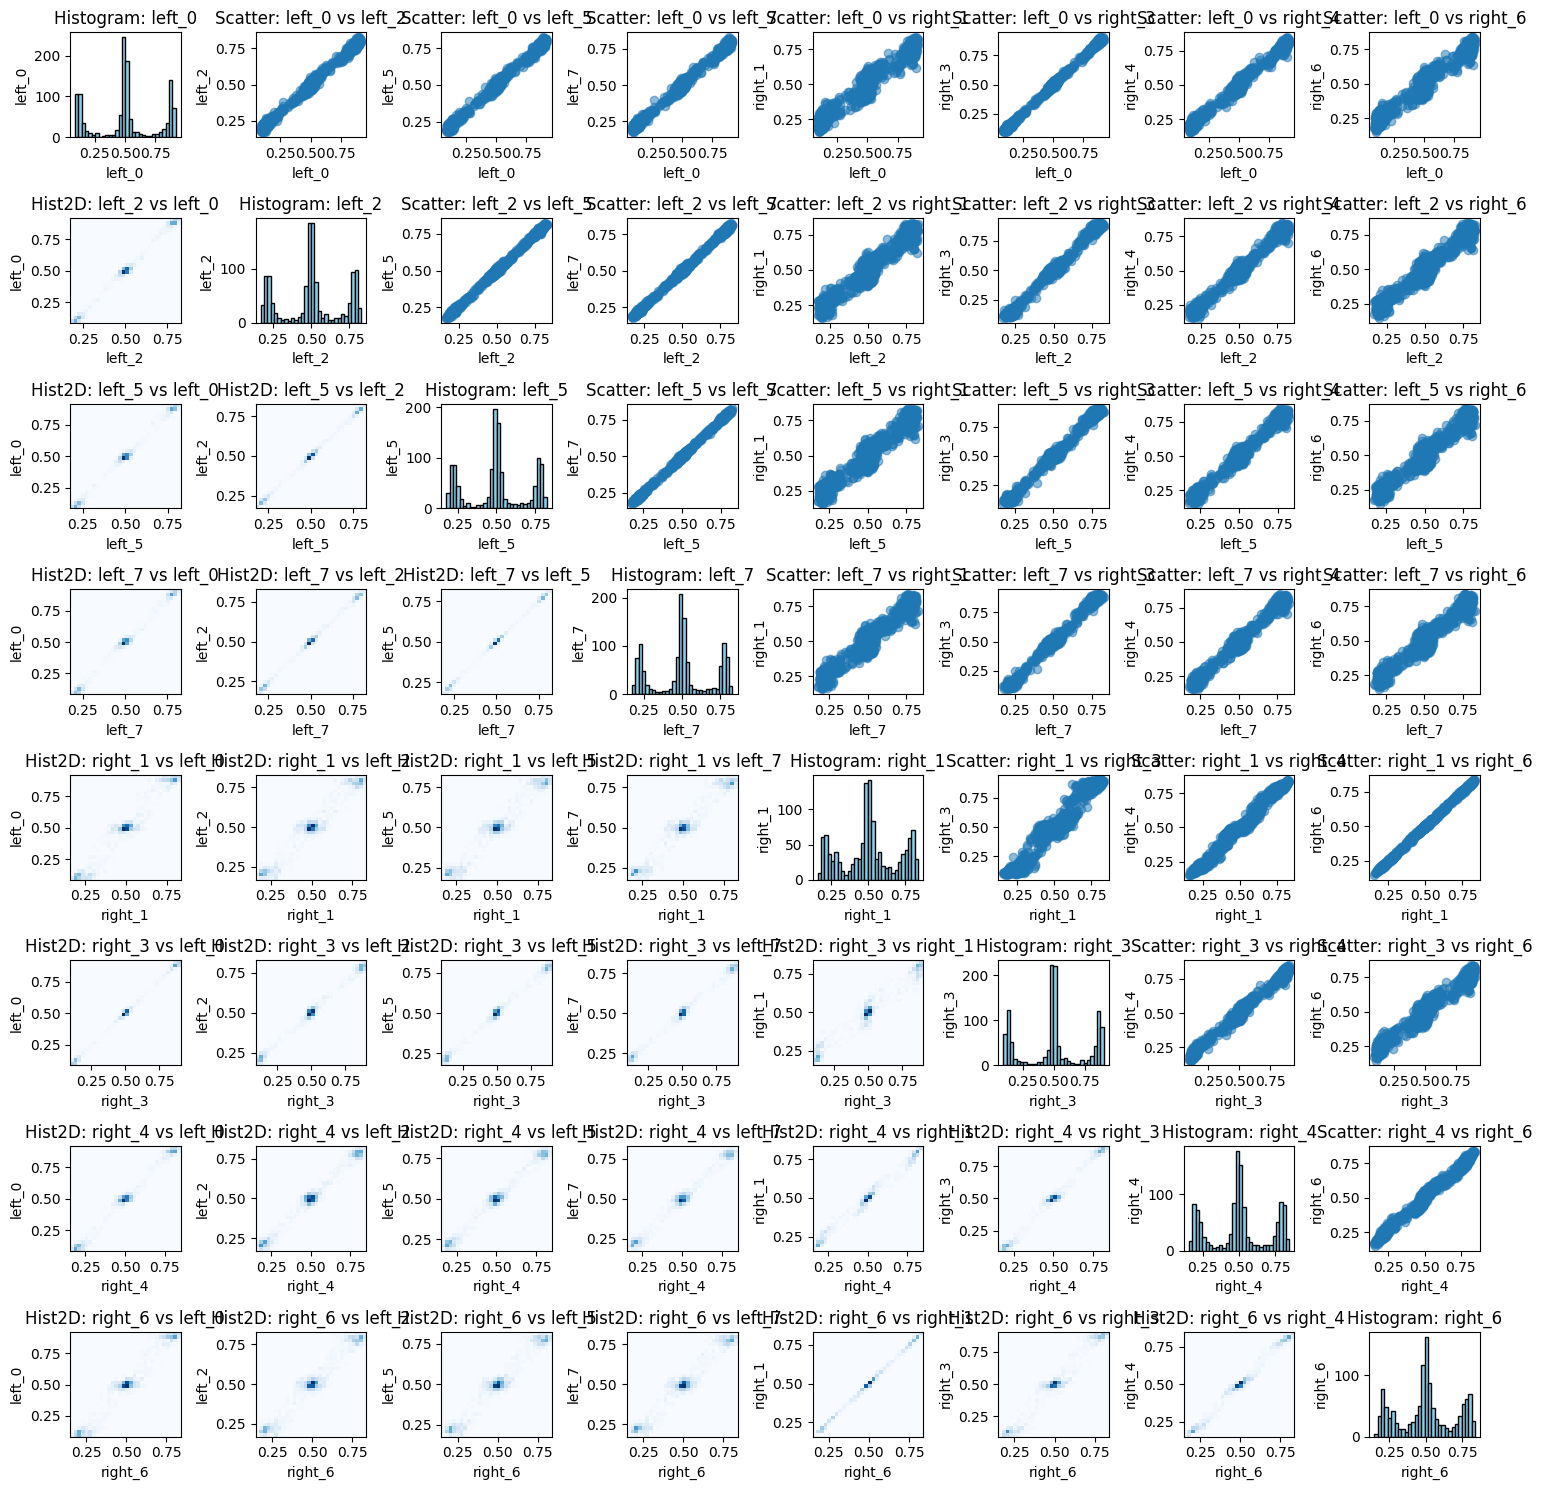
\includegraphics[width=\textwidth]{Chapter_5/figures/sensitivity_selective_advantage2.png}
%     \caption{correlation scatter plots, gland histograms and correlation heatmaps for $s=0.2$.}
%     \label{fig:sensitivity_selective_advantage2}
% \end{figure}
% \begin{figure}[h]
%     \centering
%     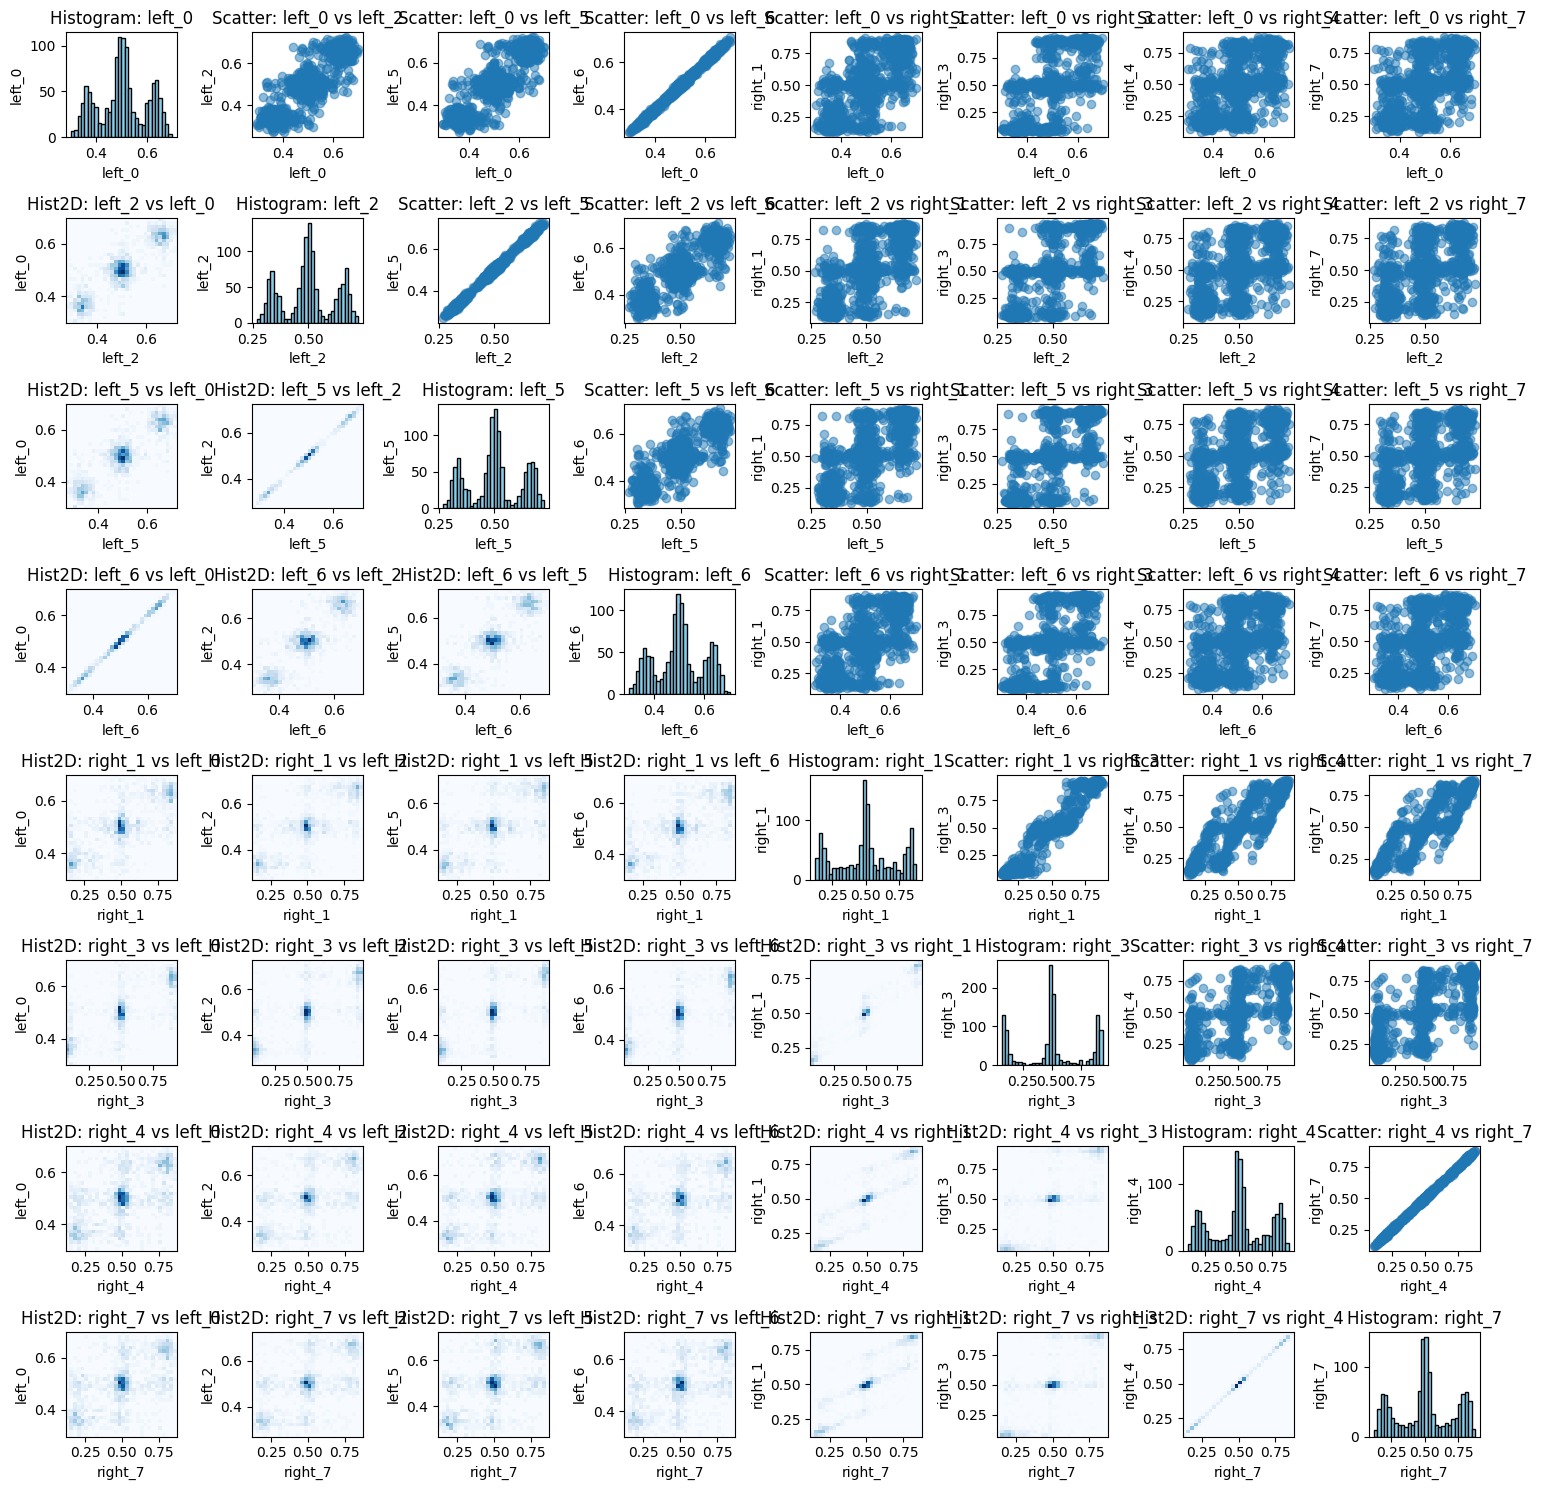
\includegraphics[width=\textwidth]{Chapter_5/figures/sensitivity_selective_advantage3.png}
%     \caption{correlation scatter plots, gland histograms and correlation heatmaps for $s=0.3$.}
%     \label{fig:sensitivity_selective_advantage3}
% \end{figure}
% In addition to the fully neutral model not recapitulating the patterns observed in data, it seems the weak selection regimes have a similarly hard time establishing lineages which would lead to decoupling between sides of the tumour.
% \clearpage
% \subsection{Driver mutation rates}
% The driver mutation rates were tested at $10^{-6}$ and $10^{-4}$ with the other parameters kept at values given in table \ref{tab:parameters}, and the case for the mutation rate equal to $10^{-5}$ covered in figure \ref{fig:sensitivity_selective_advantage3}.
% \begin{figure}[h]
%     \centering
%     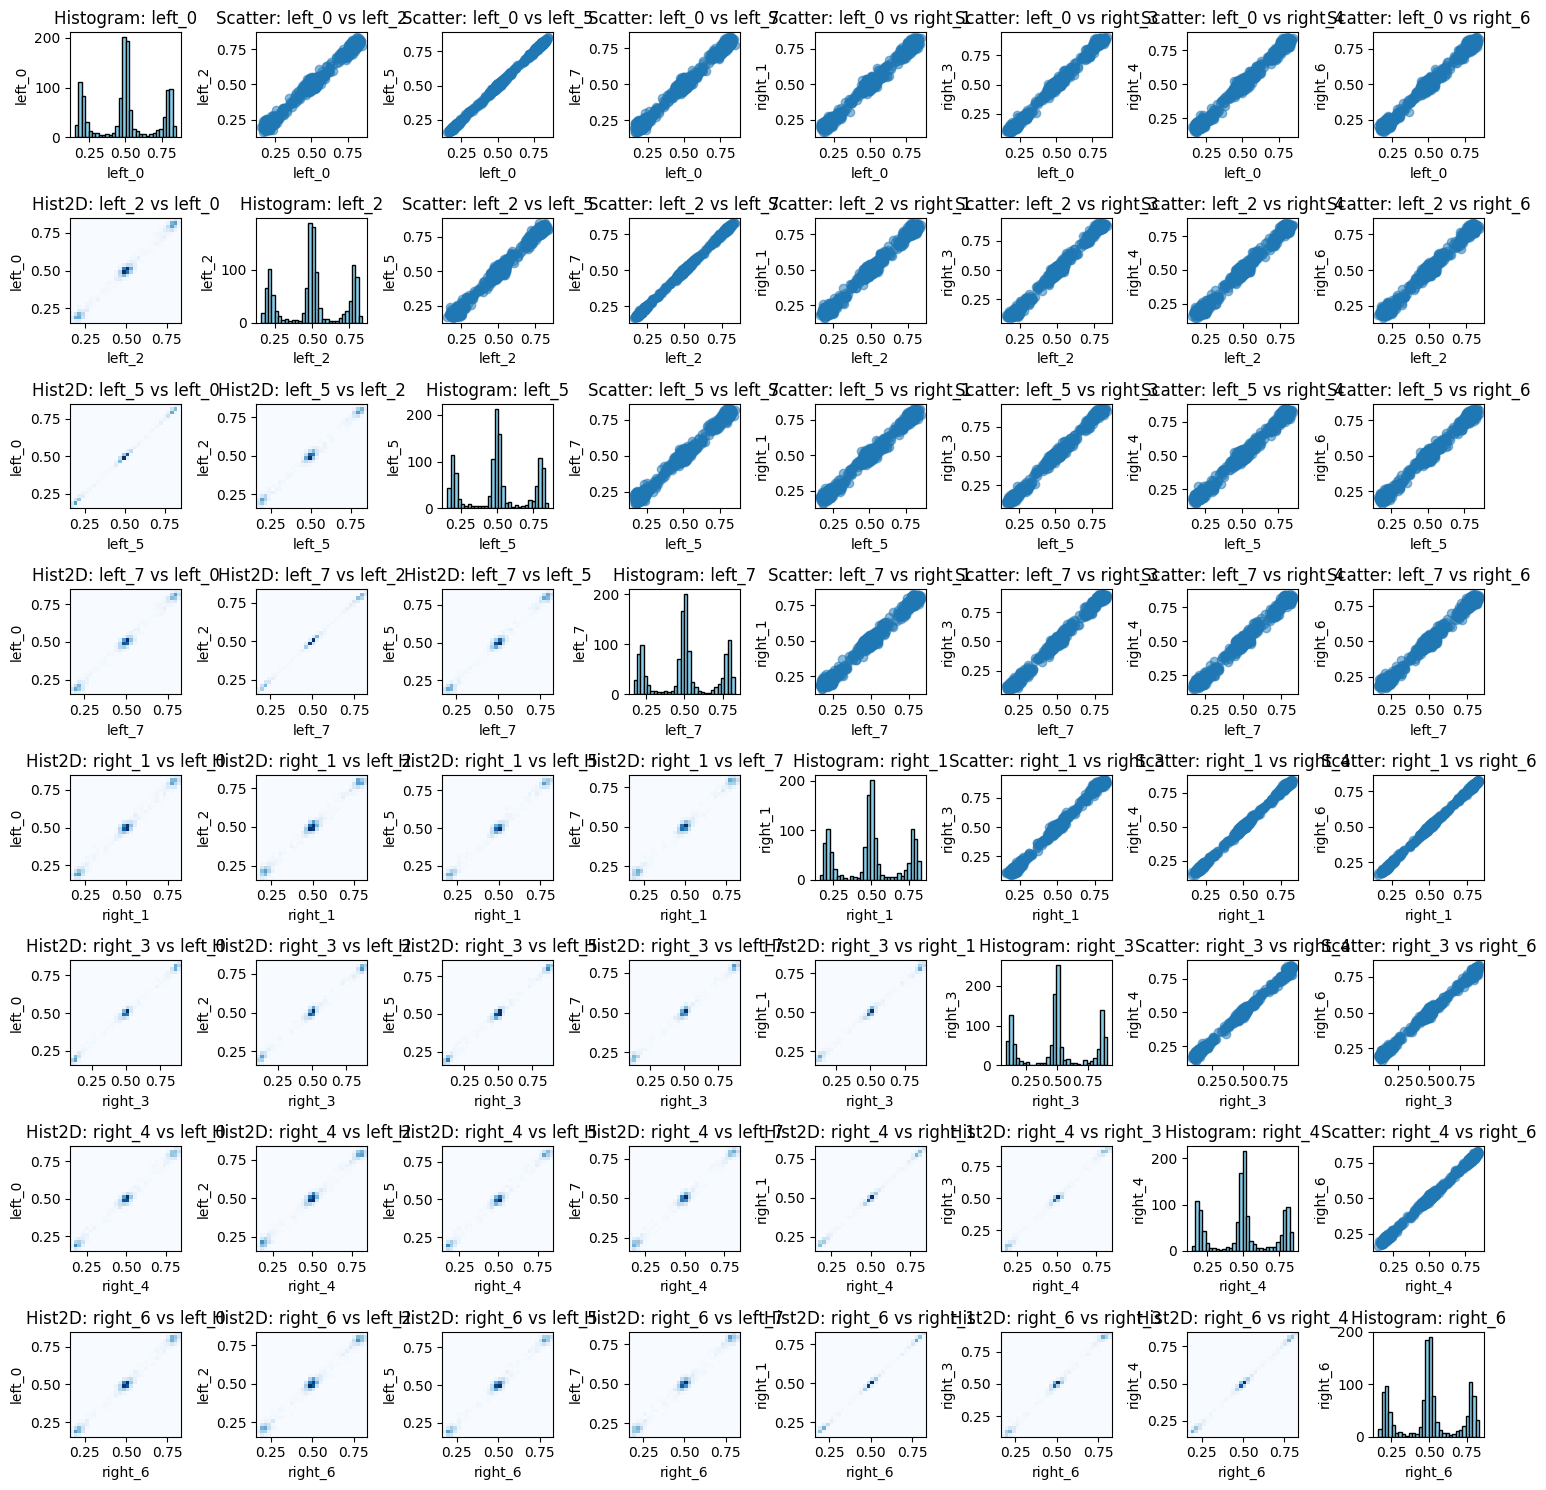
\includegraphics[width=\textwidth]{Chapter_5/figures/sensitivity_driver1.png}
%     \caption{correlation scatter plots, gland histograms and correlation heatmaps for driver mutation rate $10^{-6}$.}
%     \label{fig:sensitivity_driver1}
% \end{figure}
% \begin{figure}[h]
%     \centering
%     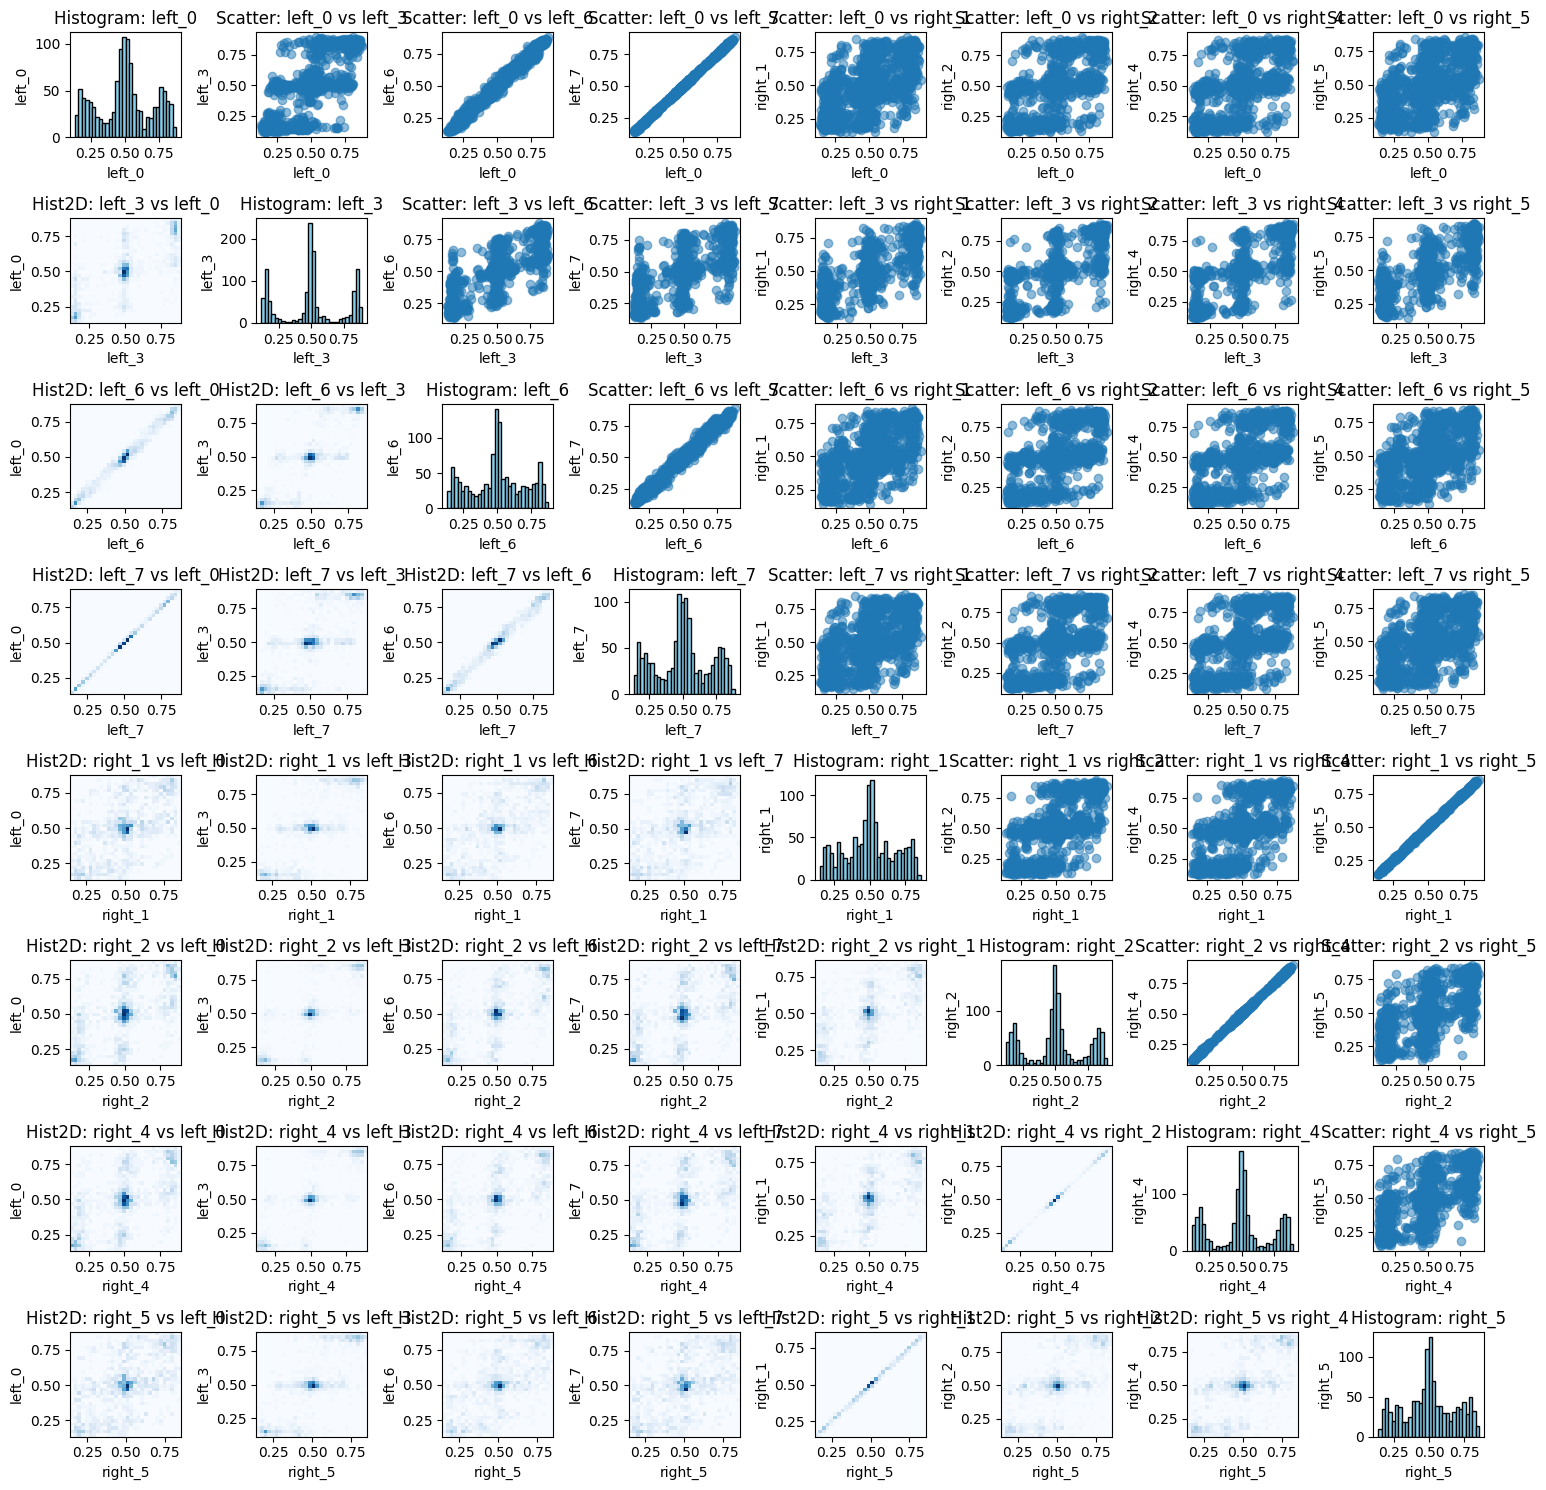
\includegraphics[width=\textwidth]{Chapter_5/figures/sensitivity_driver2.png}
%     \caption{correlation scatter plots, gland histograms and correlation heatmaps for driver mutation rate $10^{-4}$.}
%     \label{fig:sensitivity_driver2}
% \end{figure}
% \clearpage
% \subsection{fCpG flipping probabilities}
% The fCpG flipping probabilities were tested at $10^{-4}$, $10^{-3}$, and $10^{-2}$ with the other parameters as in table \ref{tab:parameters}. The case for $5\times10^{-3}$ is covered by figure \ref{fig:sensitivity_selective_advantage3}. \par
% \begin{figure}[h]
%     \centering
%     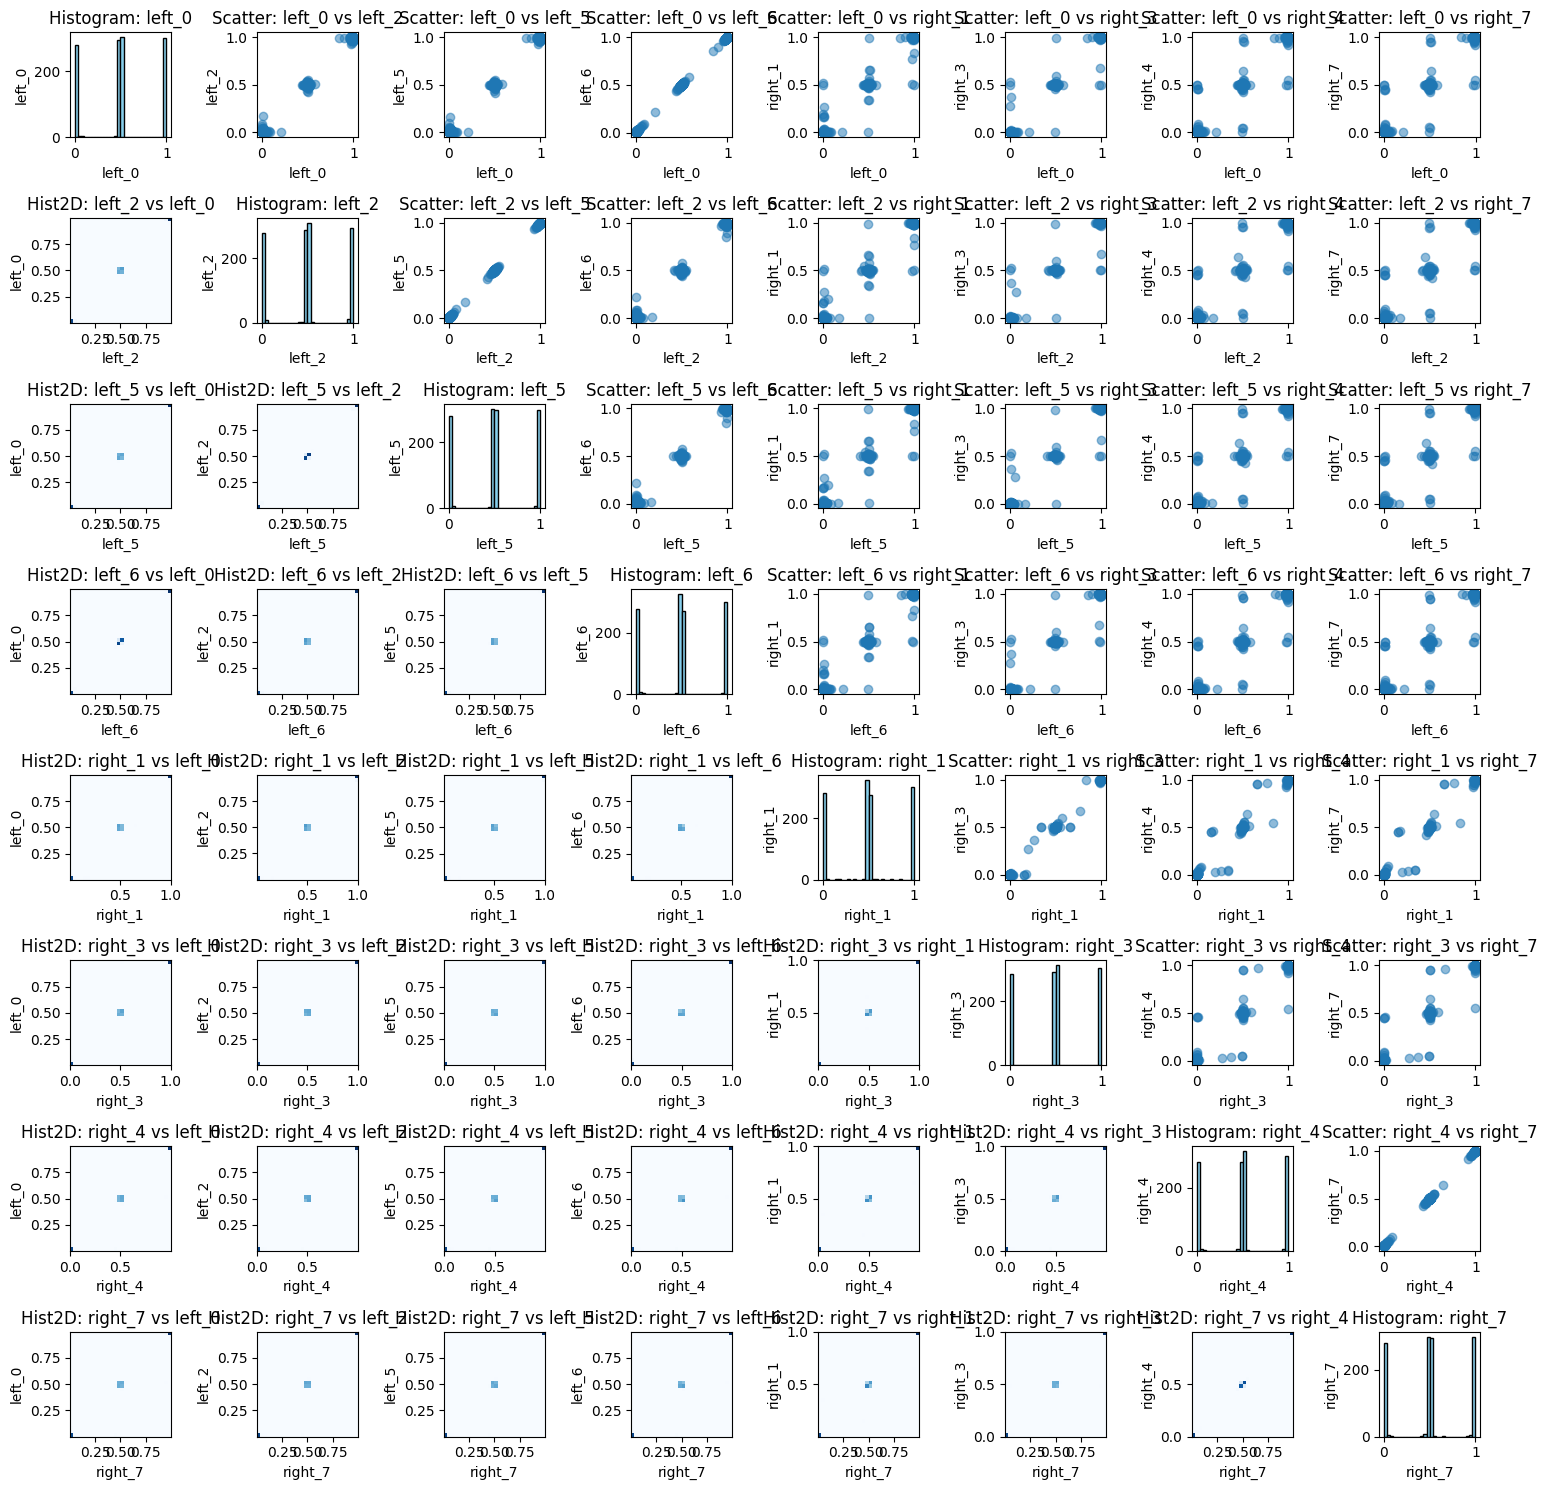
\includegraphics[width=\textwidth]{Chapter_5/figures/sensitivity_flipprob1.png}
%     \caption{correlation scatter plots, gland histograms and correlation heatmaps for flip probabilities $10^{-4}$.}
%     \label{fig:sensitivity_flipprob1}
% \end{figure}
% \begin{figure}[h]
%     \centering
%     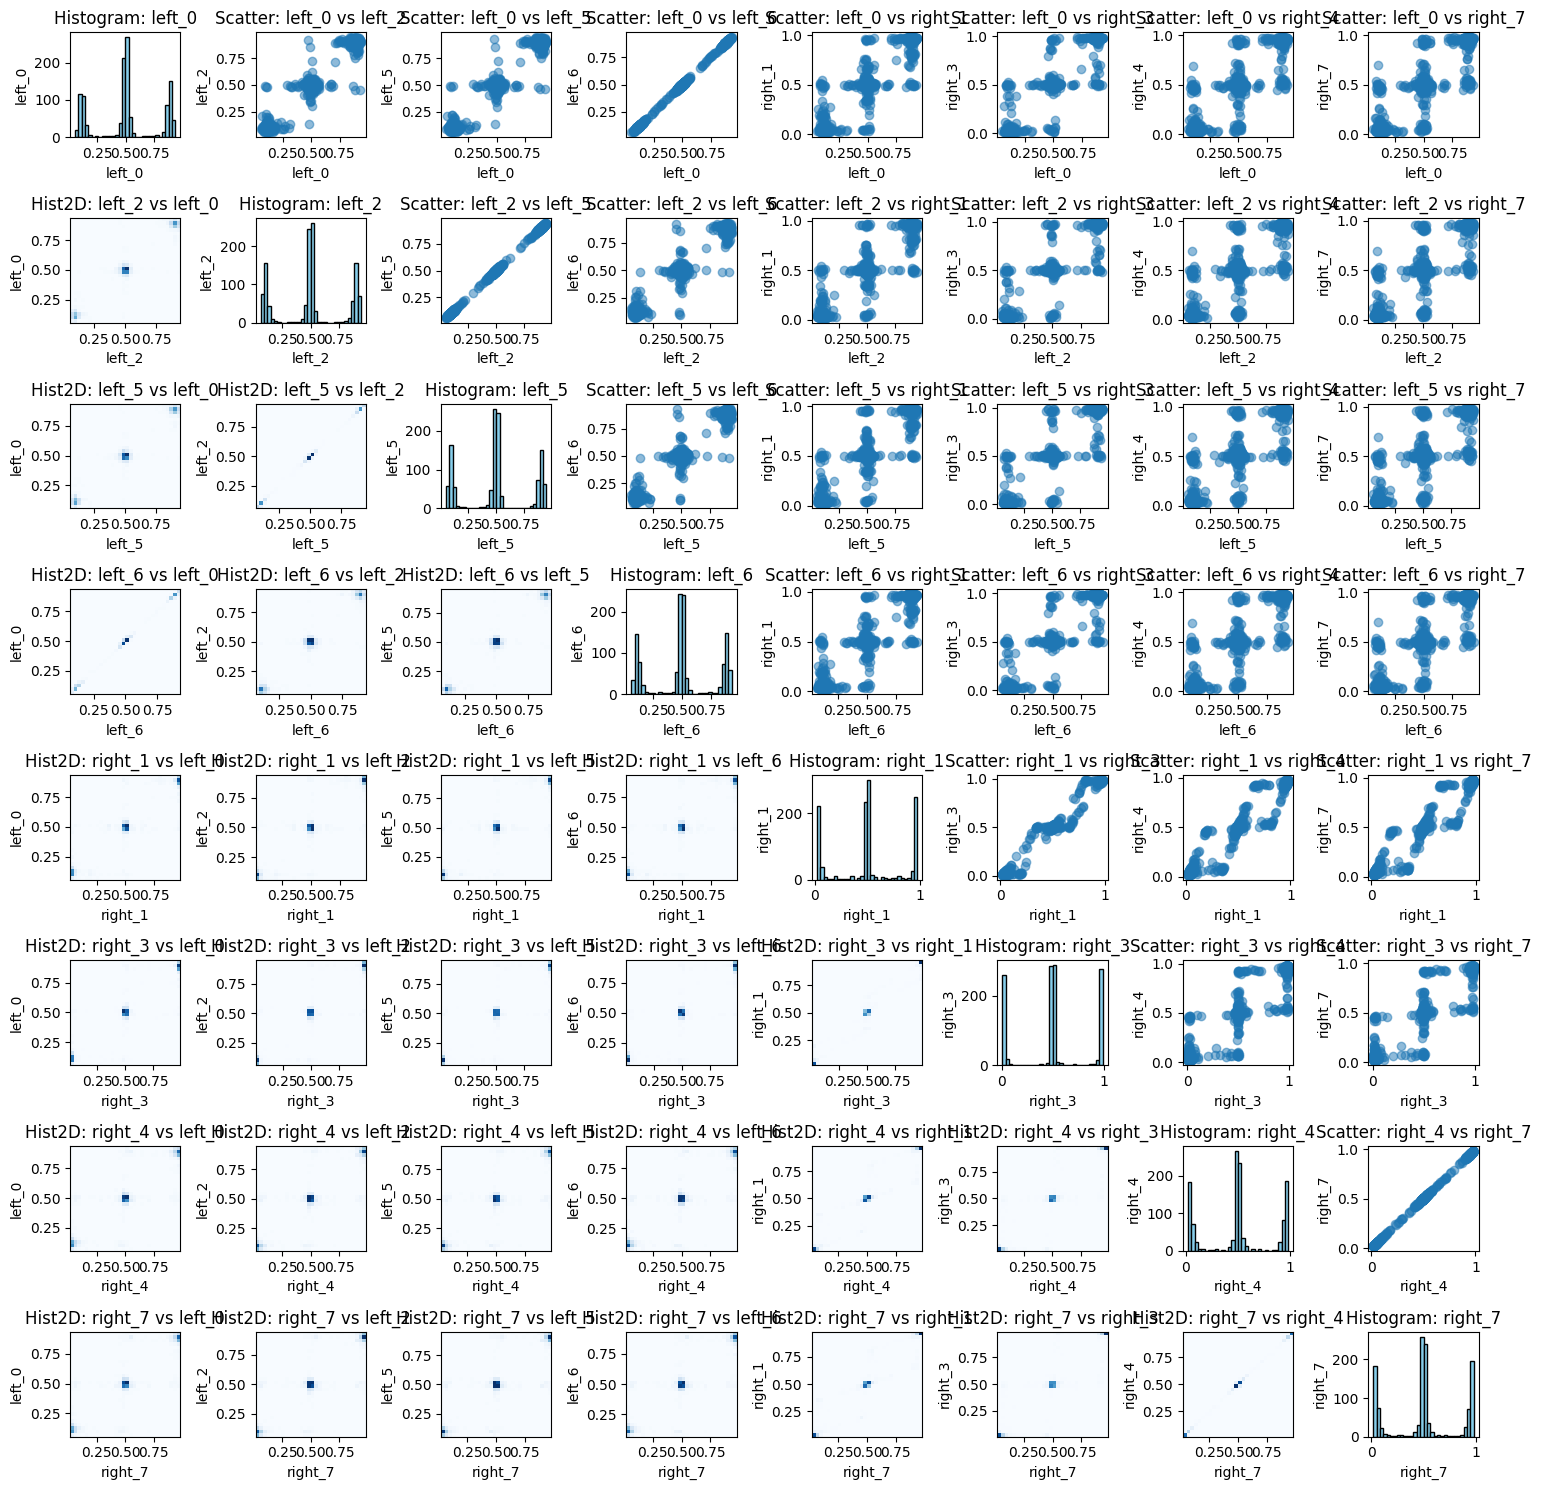
\includegraphics[width=\textwidth]{Chapter_5/figures/sensitivity_flipprob2.png}
%     \caption{correlation scatter plots, gland histograms and correlation heatmaps for flip probabilities $10^{-3}$.}
%     \label{fig:sensitivity_flipprob2}
% \end{figure}
% \clearpage
% \begin{figure}[h]
%     \centering
%     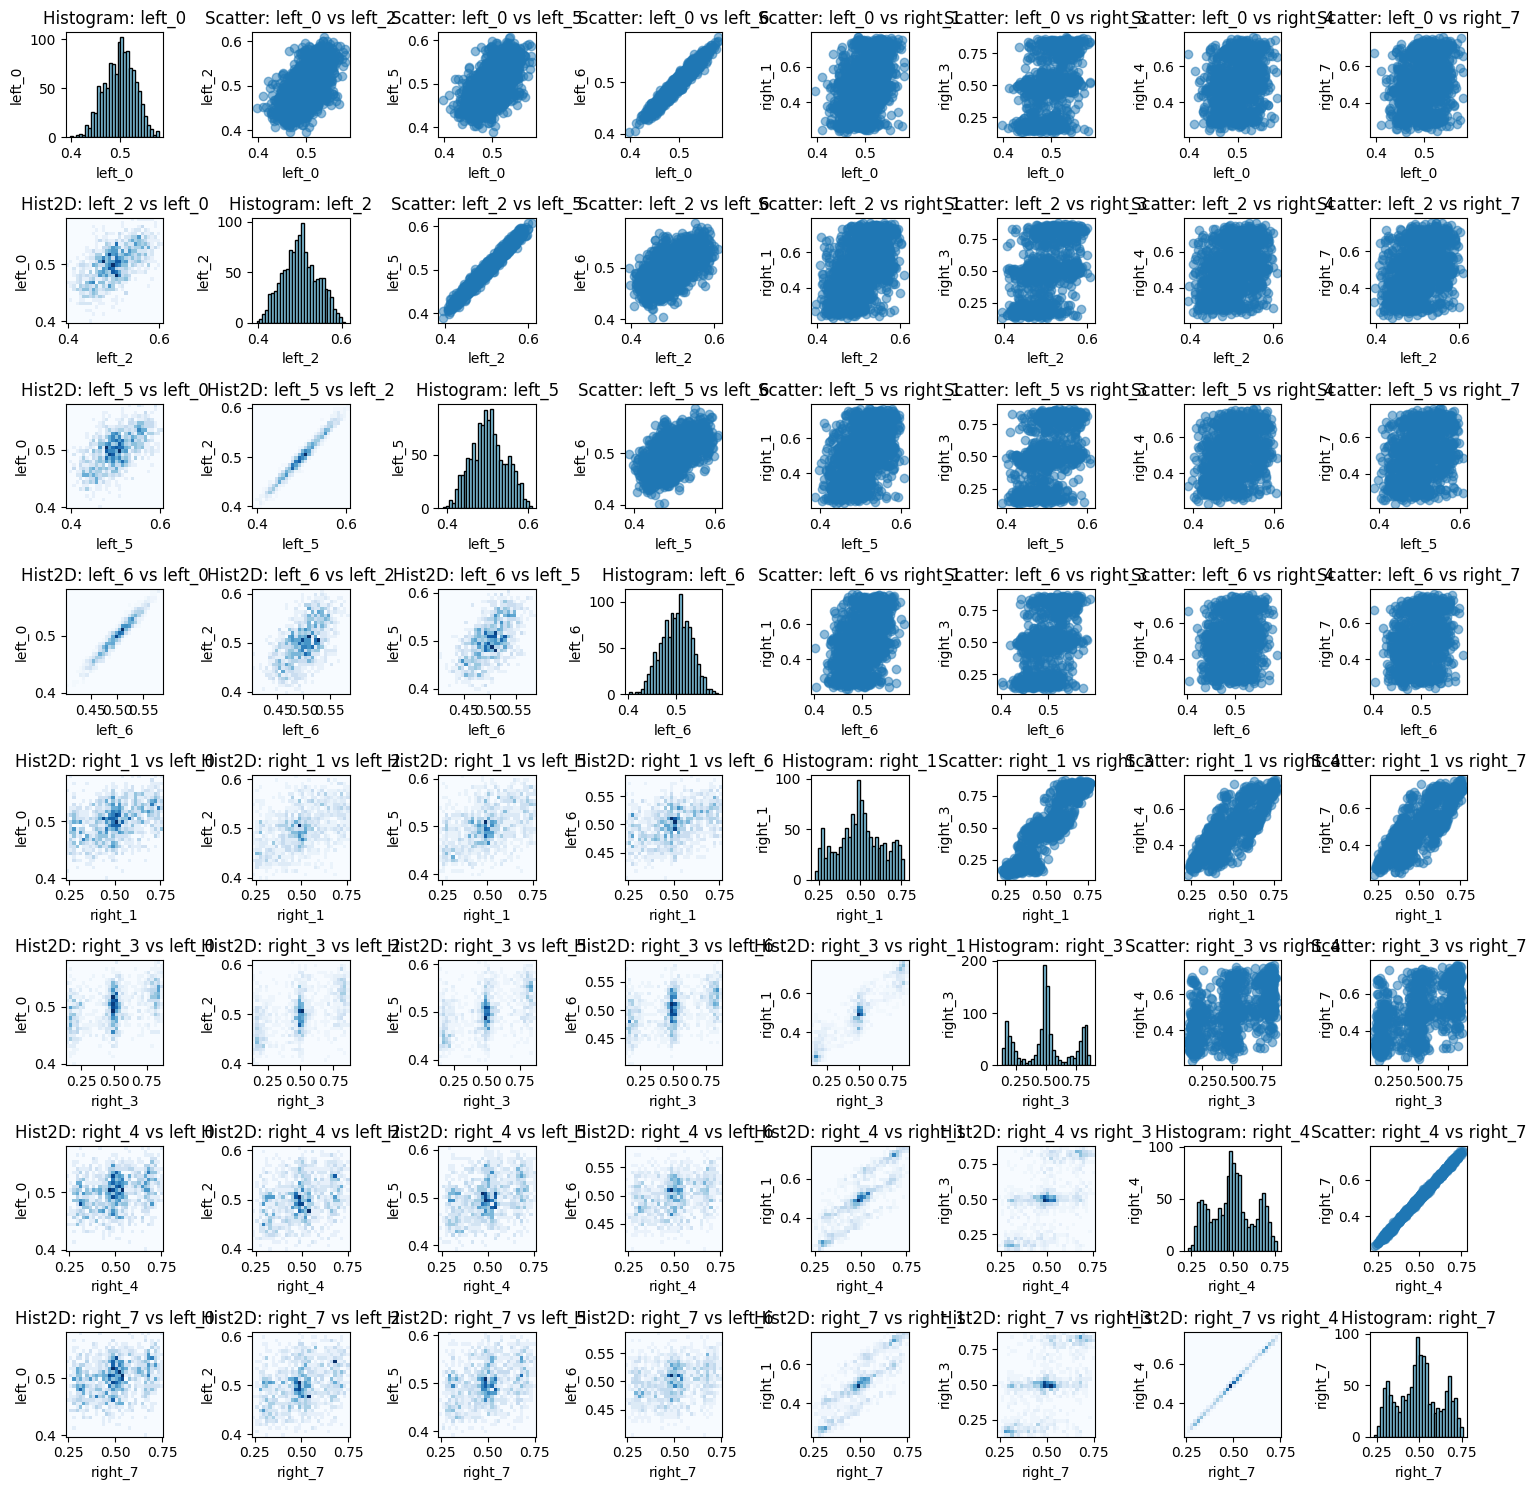
\includegraphics[width=\textwidth]{Chapter_5/figures/sensitivity_flipprob3.png}
%     \caption{correlation scatter plots, gland histograms and correlation heatmaps for flip probabilities $10^{-2}$.}
%     \label{fig:sensitivity_flipprob3}
% \end{figure}
% \clearpage
% As expected, the higher probabilities lead to quicker decoupling, even between glands which are on the same side of the tumour. On the other hand, lower probabilities show very little change between the initial and final arrays.

% \subsection{Gland fission rates}
% The gland fission rates tested were $0.008$, $0.08$, and $0.8$. The other parameters were kept as in table \ref{tab:parameters}. The case of $0.008$ did not produce any fissions and is not included below, and the case of $0.08$ had a total of $4$ fissions which resulted in $5$ glands at the end of the simulation. The case for fission rates equal to $0.4$ was covered in figure \ref{fig:sensitivity_selective_advantage3}.
% \begin{figure}[h]
%     \centering
%     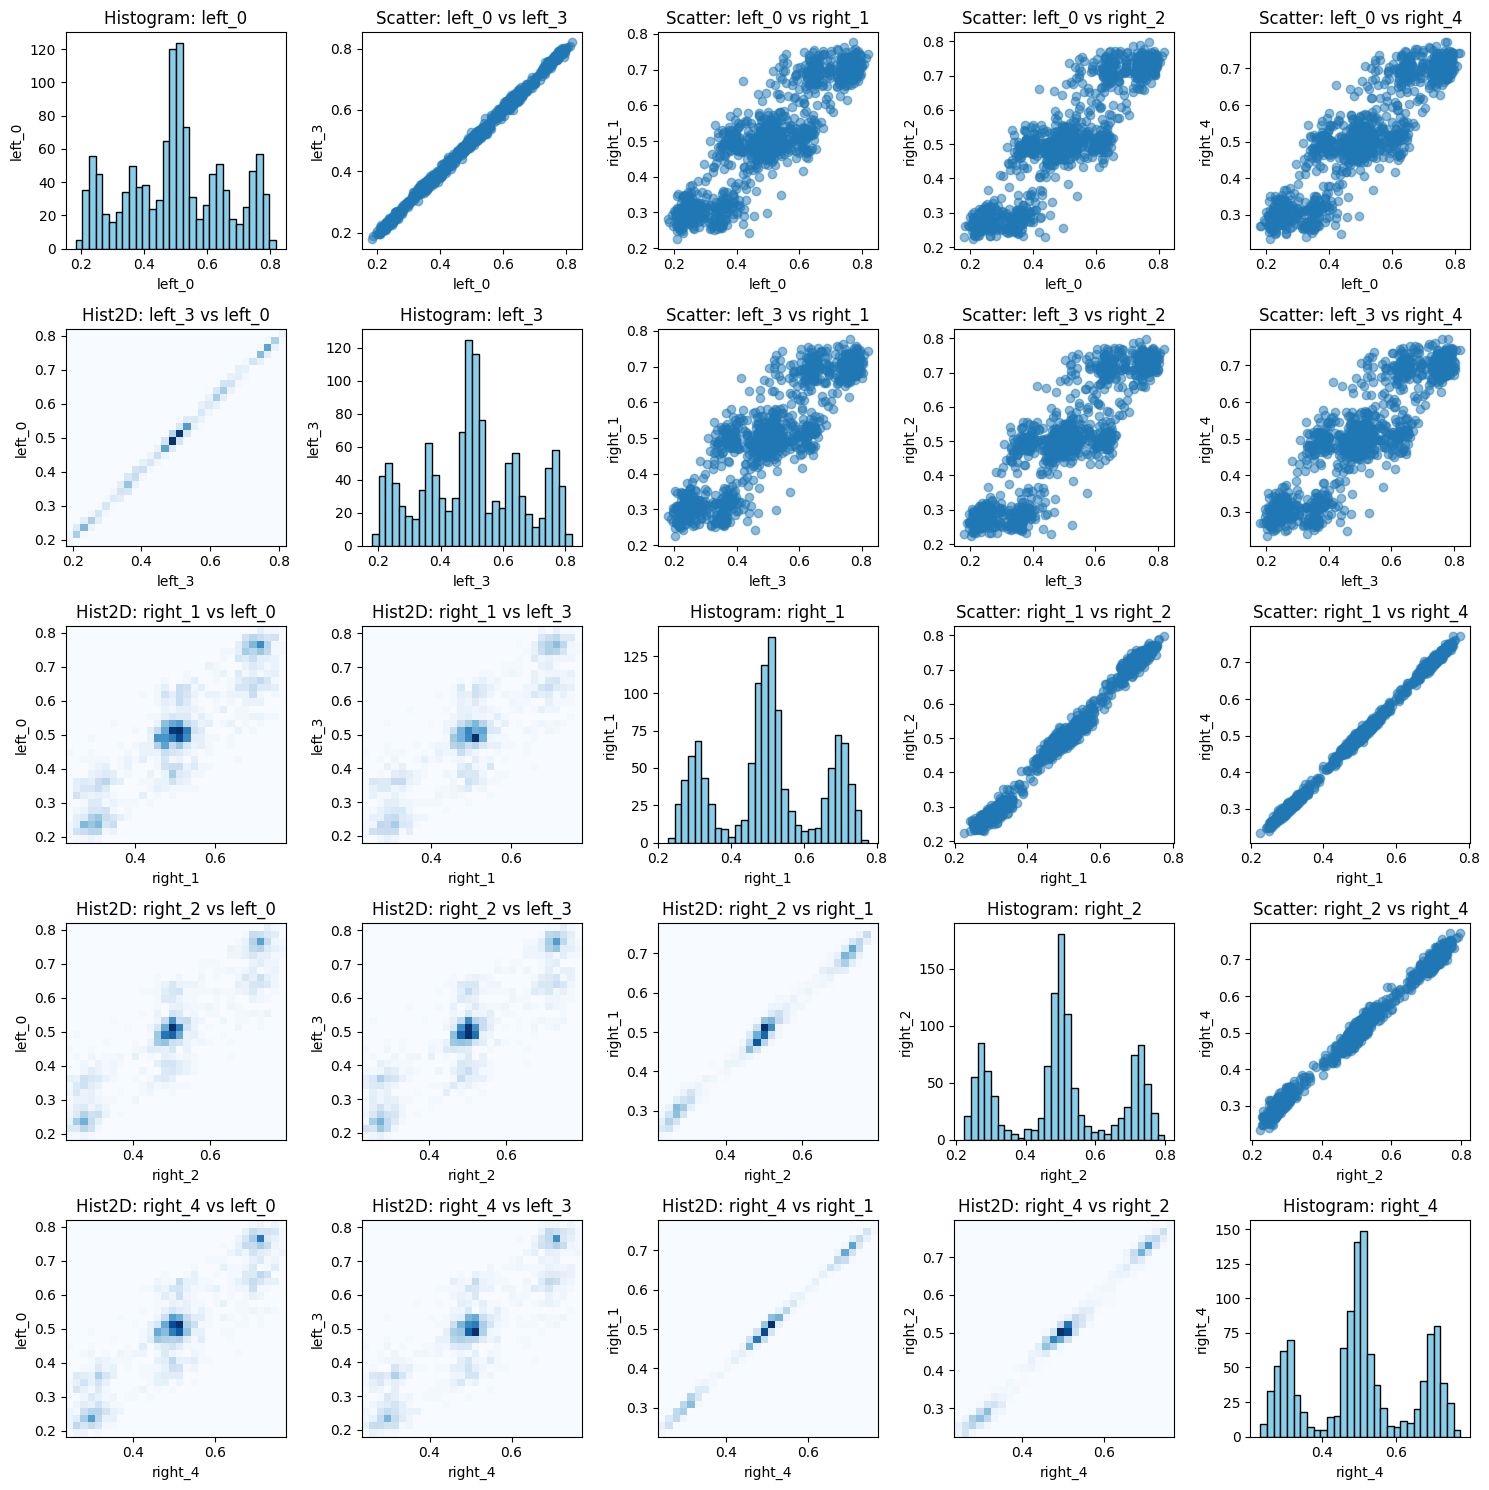
\includegraphics[width=\textwidth]{Chapter_5/figures/sensitivity_migrate1.png}
%     \caption{correlation scatter plots, gland histograms and correlation heatmaps for fission rates $0.008$.}
%     \label{fig:sensitivity_migrates1}
% \end{figure}
% \begin{figure}[h]
%     \centering
%     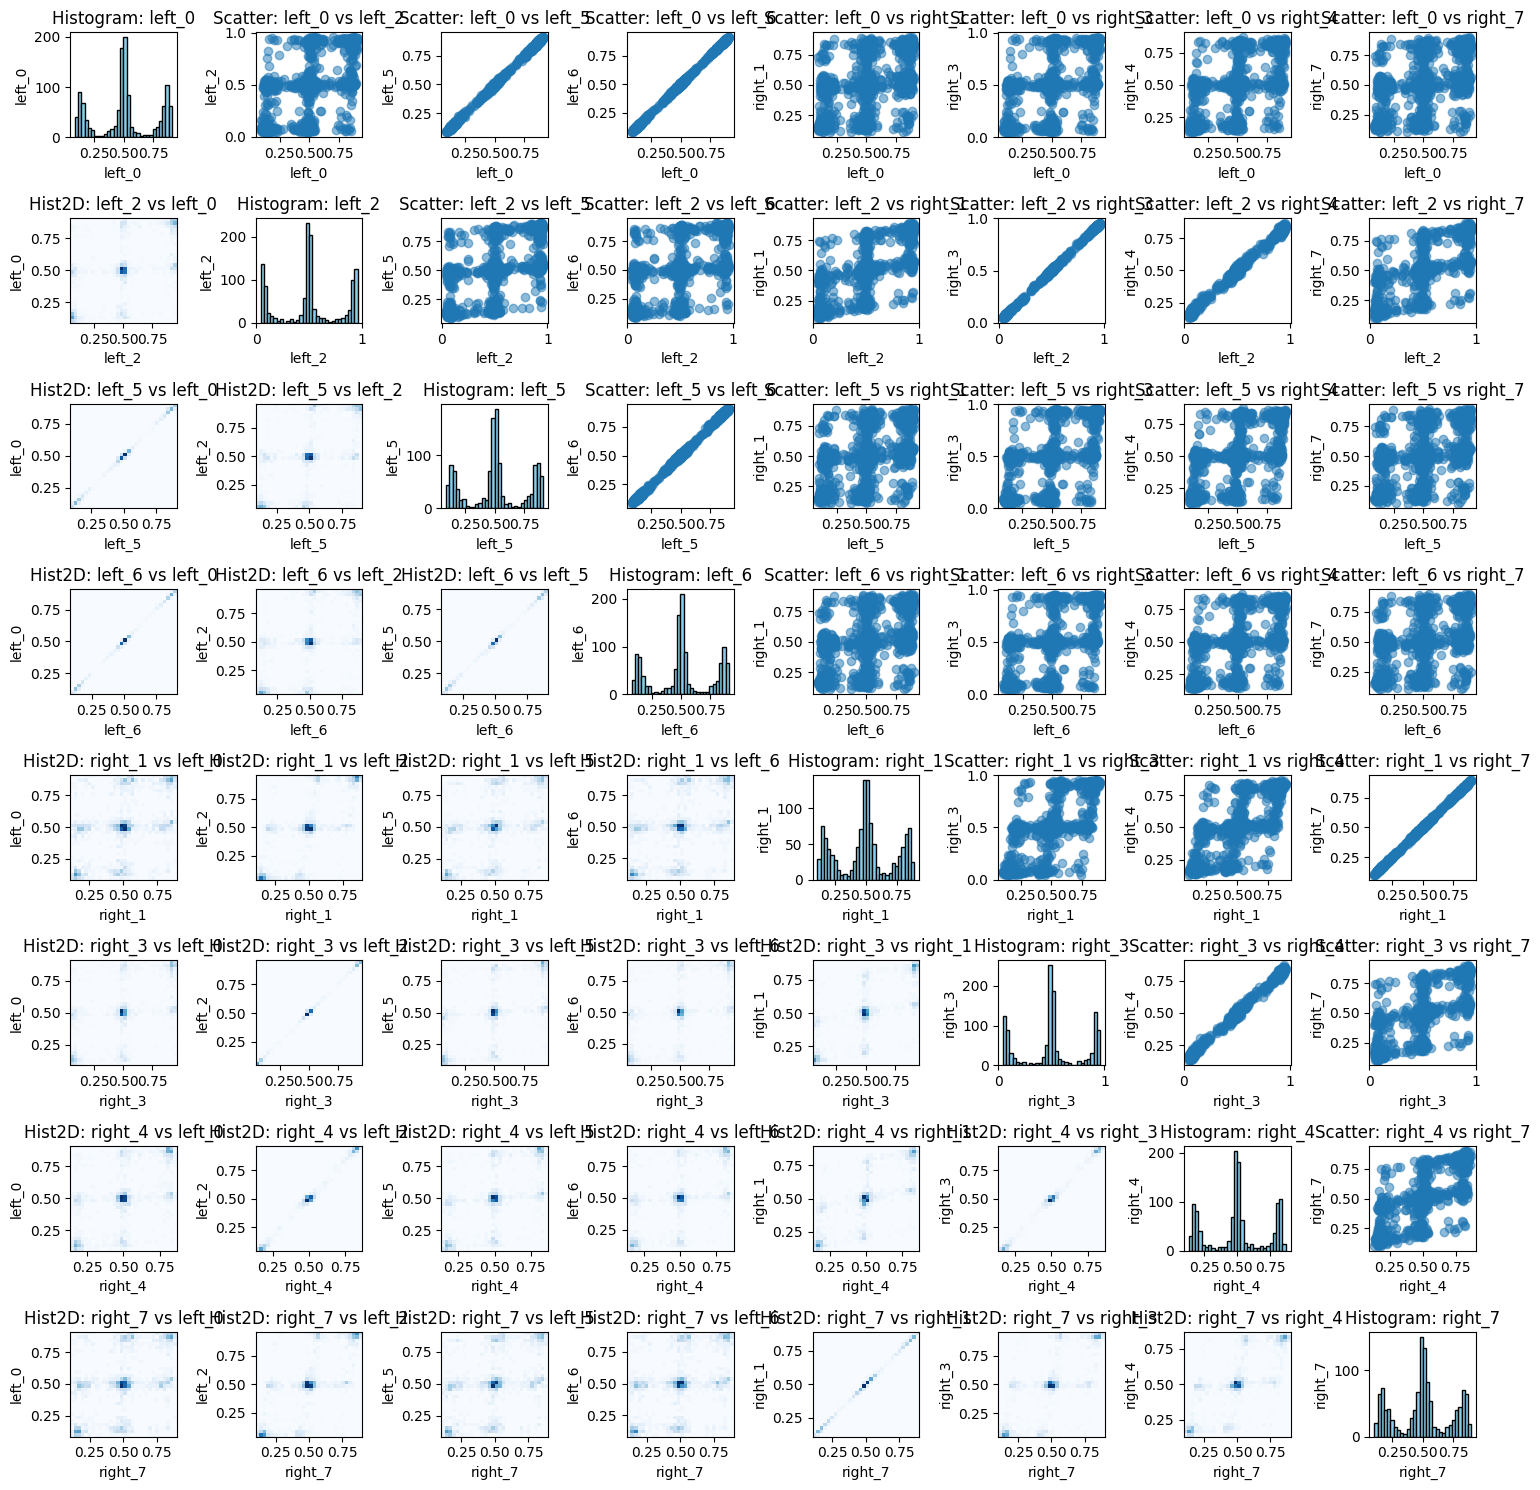
\includegraphics[width=\textwidth]{Chapter_5/figures/sensitivity_migrate2.png}
%     \caption{correlation scatter plots, gland histograms and correlation heatmaps for fission rates $0.08$.}
%     \label{fig:sensitivity_migrate2}
% \end{figure}
% \clearpage
% Nominally, faster fission rates should lead to less time spent in turnover before fission, and therefore less time for the fCpG sites to decouple. However, I set these simulations up with that in mind so that the glands spend around $40\%$ of the simulated time in turnover.

% \section{Parameters}
% The loose default parameter settings used in the simulations are given in Table \ref{tab:parameters}.

% \begin{table}[ht]
% \centering
% \begin{tabular}{|l|l|}
% \hline
% Parameter & Value \\
% \hline
%     Driver mutation rate & $10^{-5}$   \\
%     Methylation probability per fCpG site per cell division & $5\times10^{-3}$ \\
%     Demethylation probability per fCpG site per cell division & $5\times10^{-3}$ \\
%     Gland fission rate & $0.4$  \\
%     Cells per gland & 8192 \\
%     fCpG loci per cell & 1200 \\
%     Selective advantage & $0.3$ \\
% \hline
% \end{tabular}
% \caption{Default parameter values.}\label{tab:parameters}
% \end{table}
% The values are educated guesses based on the two fCpG papers. The simulations were run for $50$ Gillespie generations, which equated to tumours between 10 and 50 glands across. The tumours were allowed about $40\%$ of the growth time in turnover. The simulations were run on my laptop, I am currently scaling the framework up for deployment on City's computing cluster.\par

% \section{Distance functions}
% The basic distance functions I have started from are inspired by the Metropolitan distance. The distance between site $A$ in gland $2$ and site $A$ in gland $2$ is calculated as the classic Metropolitan distance with a modification that the values of $A_1$ and $A_2$ are put in bins based on their proximity to the values of $0$, $0.5$, and $1$. The main difference between distance functions I've experimented with is adjusting the value added to the distance based on the difference between sites in different glands.
% \begin{figure}[h]
%     \centering
%     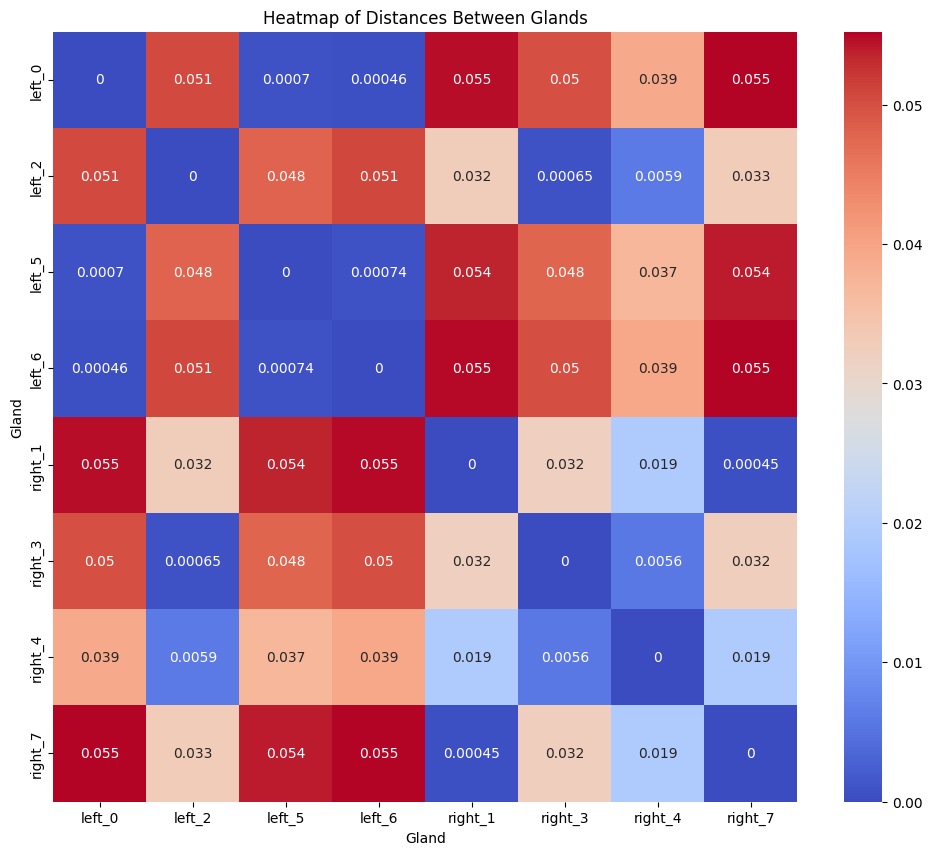
\includegraphics[width=\textwidth]{Chapter_5/figures/sensitivity_migrate2_distances.png}
%     \caption{Distances between glands from figure \ref{fig:sensitivity_migrate2}.}
%     \label{fig:distance_functions}
% \end{figure}
% \begin{figure}[h]
%     \centering
%     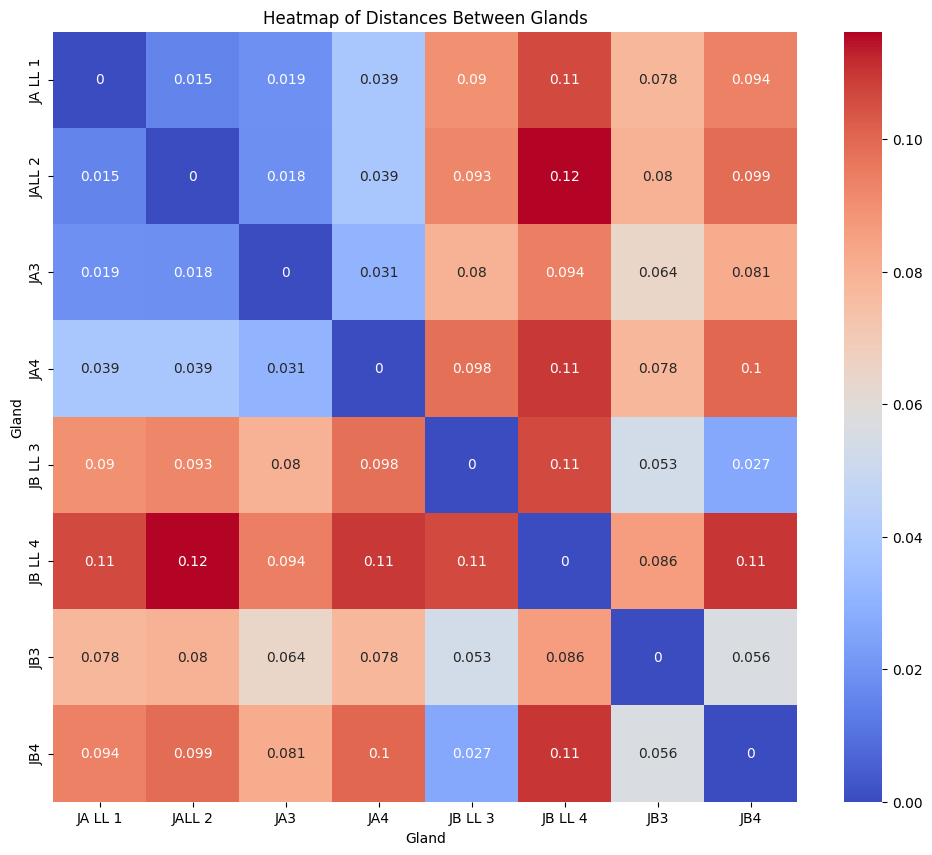
\includegraphics[width=\textwidth]{Chapter_5/figures/data_example_distances.png}
%     \caption{Distances between glands from data set J.}
%     \label{fig:data_distances}
% \end{figure}
% \begin{figure}[h]
%     \centering
%     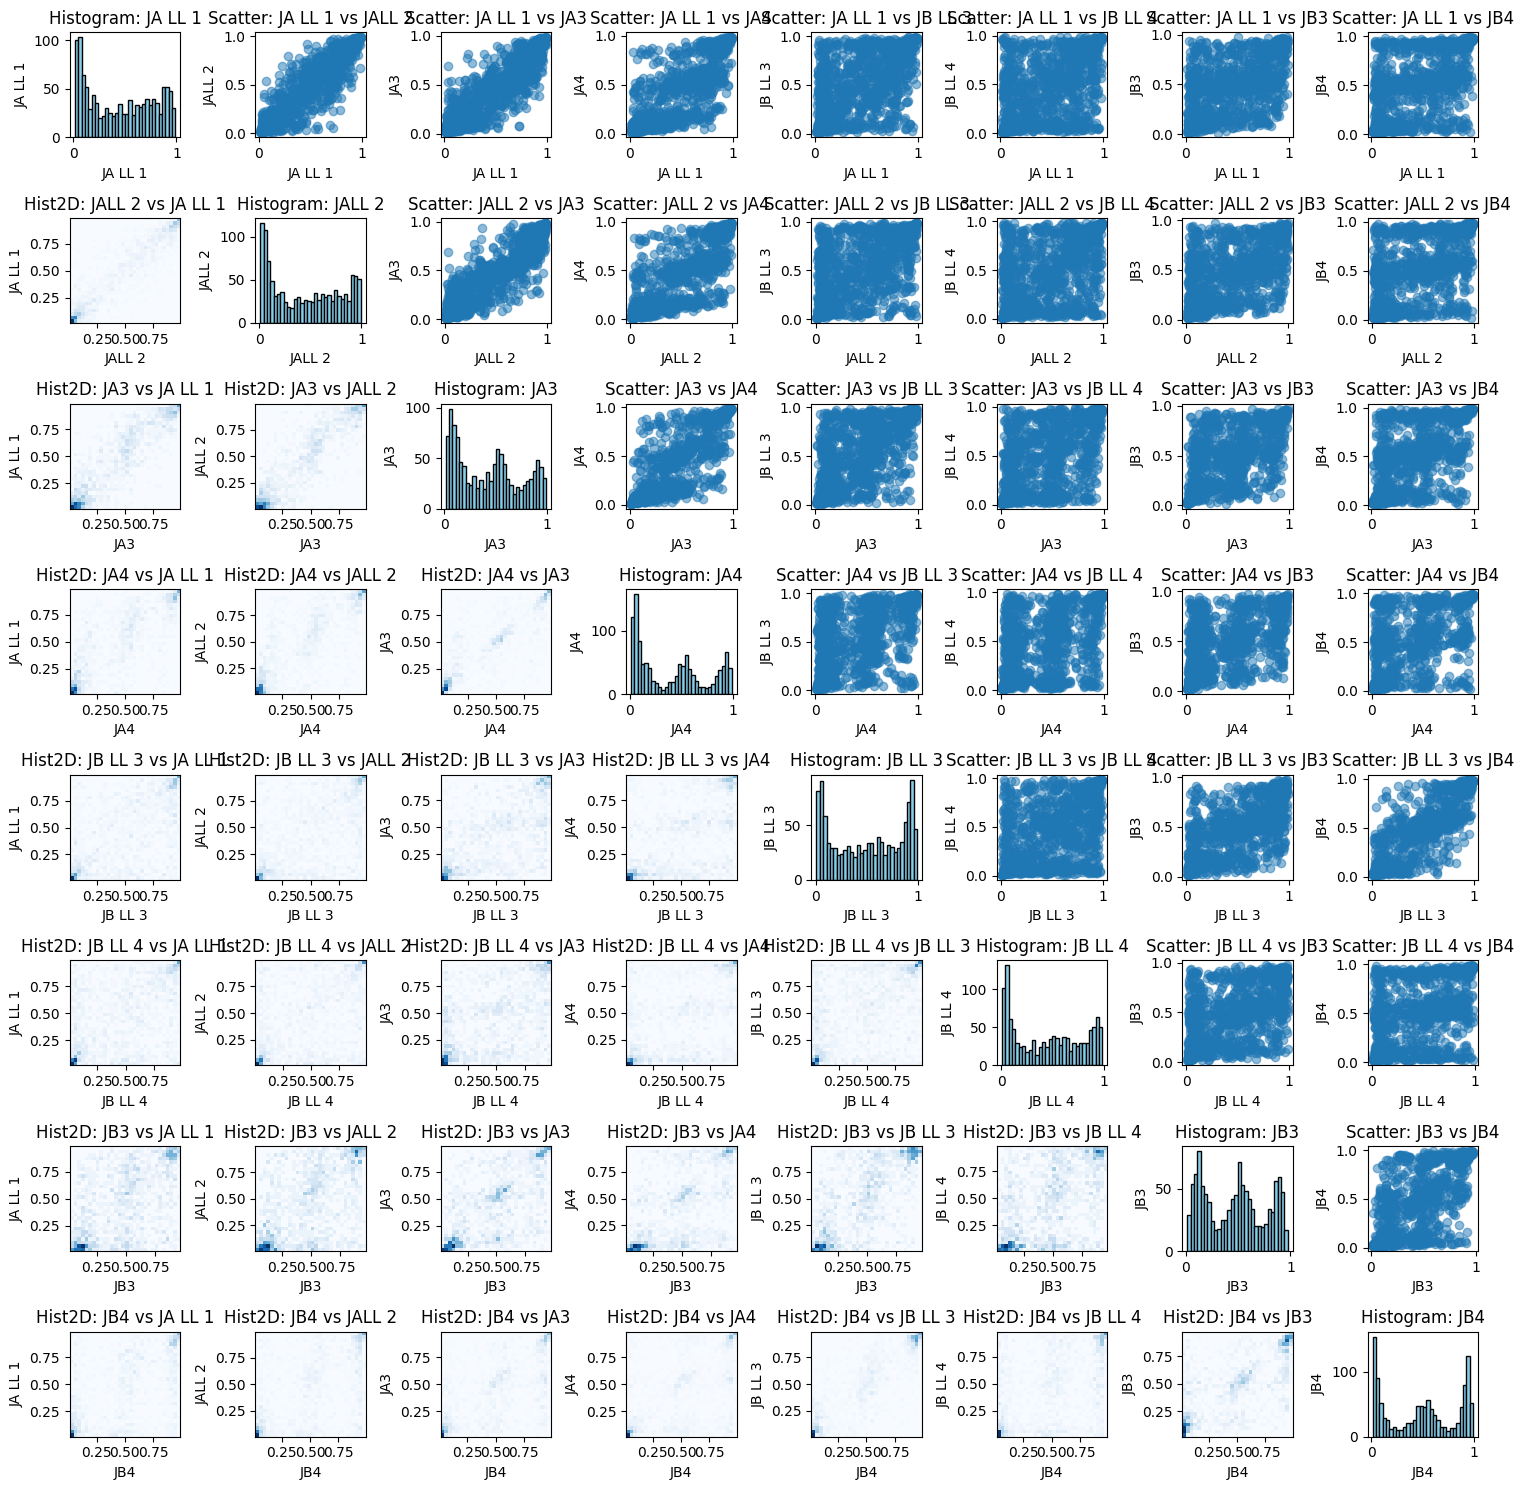
\includegraphics[width=\textwidth]{Chapter_5/figures/data_example_corrs.png}
%     \caption{Data set J whose distances are shown in \ref{fig:data_distances}.}
%     \label{fig:data_example_corrs}
% \end{figure}
% \clearpage
% \section{Next steps/work in progress}
% Currently working on the following:
% \begin{itemize}
%     \item Grid search over the above parameter space to check whether there are clusters which correspond to different tumour growth regimes.
%     \item Refining the distance functions to better capture the differences between the arrays.
% \end{itemize}
% Next on the list:
% \begin{itemize}
%     \item Inferring parameters from synthetic data based on the above two steps.
%     \item Inference of parameters or qualitative properties of real data sets - depends on the results of the above.
% \end{itemize}

% \subsection{Hypotheses}
% \begin{itemize}
%     \item \texttt{methdemon} recapitulates FMC patterns in colorectal cancer. \textbf{Test:} Extensive sensitivity analysis of \texttt{methdemon} and comparison to a different model (A/B model test with a simpler model, rule out trivial and, ideally, non-trivial models).
%     \item \texttt{methdemon} reproduces evolutionary dynamics of colorectal cancer (effectively neutral). \textbf{Test:} Inferring parameters from simulations --- under consideration are fission rate, mutation rate, time under turnover.
%     \item stem cell hypothesis - assume expansion process for each lineage and draw all cells within glands from distribution (multinomial or whatever). polyclonal origin - easy to test (fully neutral).
%     \item Spatial resolution is needed to recover evolutionary dynamics of colorectal cancer. \textbf{Test:} Compare \texttt{methdemon} to EVOFLUx (average over the data for each cancer to run the latter).
%     \item FMC patterns imply evolutionary bottlenecks between distant glands in colorectal cancer. \textbf{Test:} Develop distance metric, run EVOFLUx on individual glands (or a variation of EVOFLUx). NOTE: ask Darryl if he can be more specific on which bottlenecks he means. Need specific things that can be implemented in the model.
% \end{itemize}

